\chapter{APPENDIX A}

\begin{figure}[h]
\centering
\subfigure[PDR]{
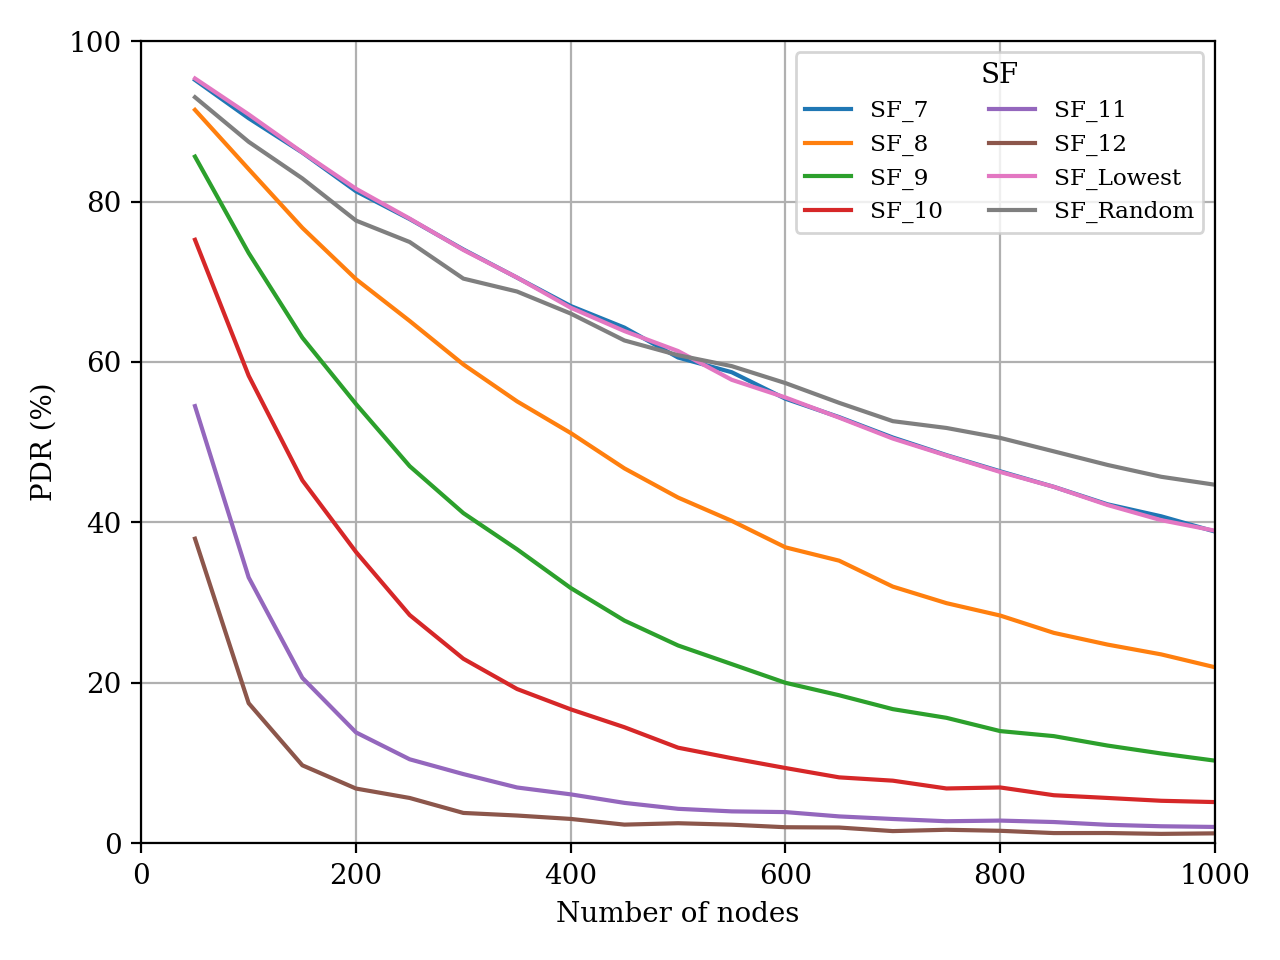
\includegraphics[width=.43\linewidth]{{fig/appendix/sf_pdr_r3000_g1_p0.01_s3600}.png}}
\subfigure[Transmit energy]{
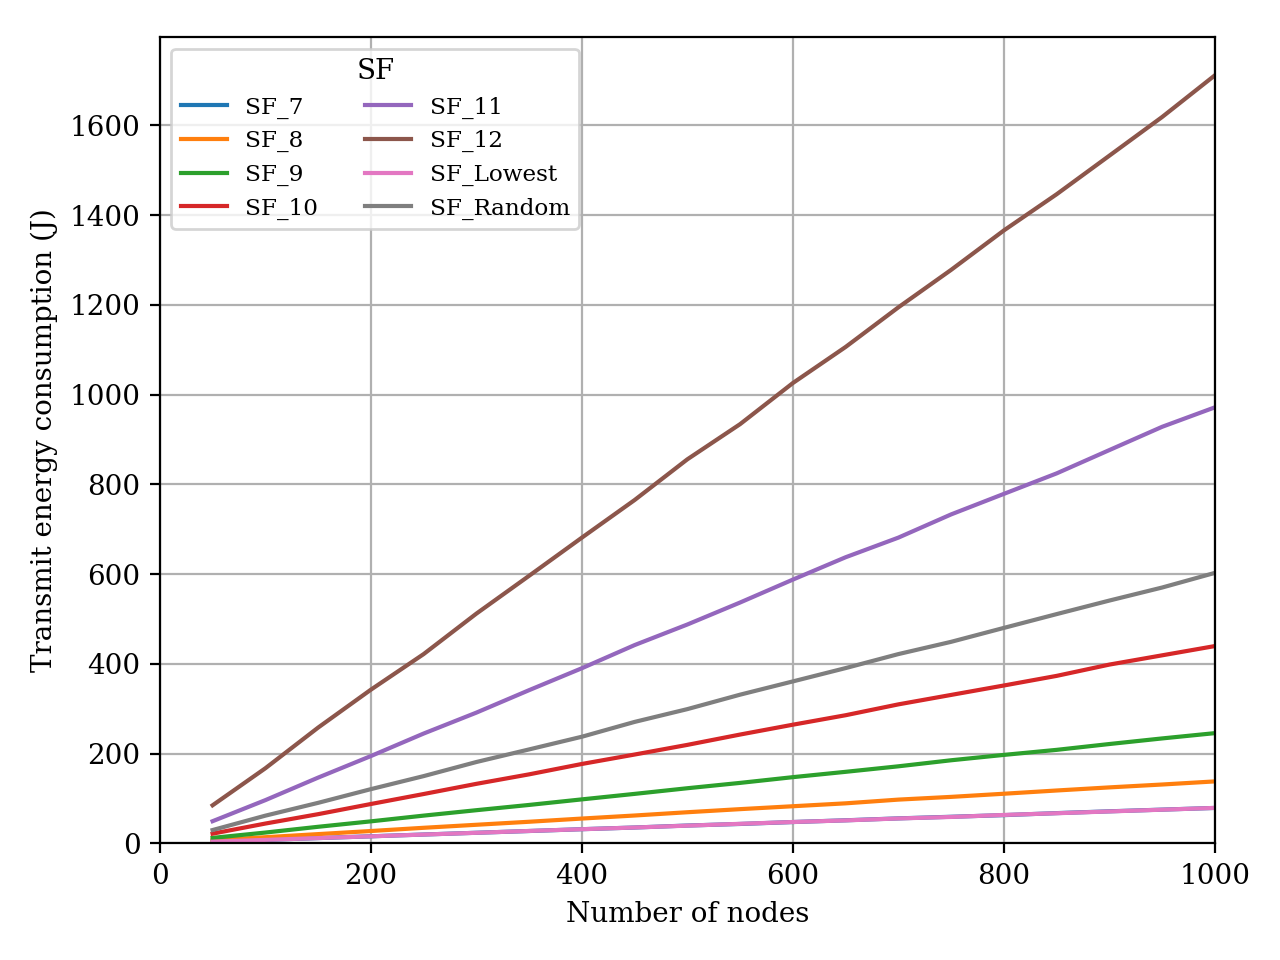
\includegraphics[width=.43\linewidth]{{fig/appendix/sf_energy_r3000_g1_p0.01_s3600}.png}}
\caption{(r = 3000 m, GW = 1)}
\label{fig:sf_r3000_g1}
\end{figure}

\begin{figure}[h]
\centering
\subfigure[PDR]{
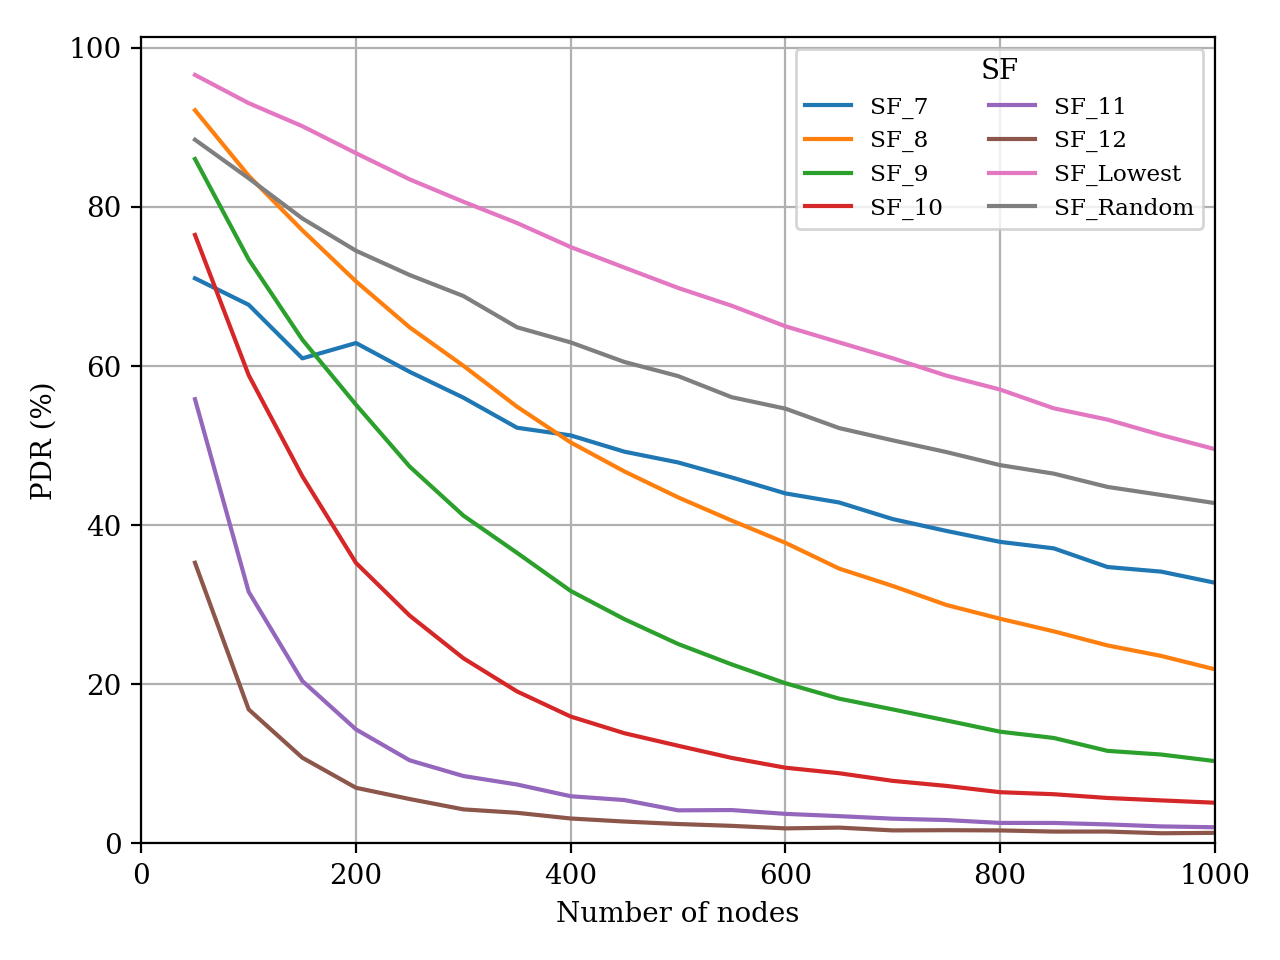
\includegraphics[width=.43\linewidth]{{fig/appendix/sf_pdr_r5000_g1_p0.01_s3600}.png}}
\subfigure[Transmit energy]{
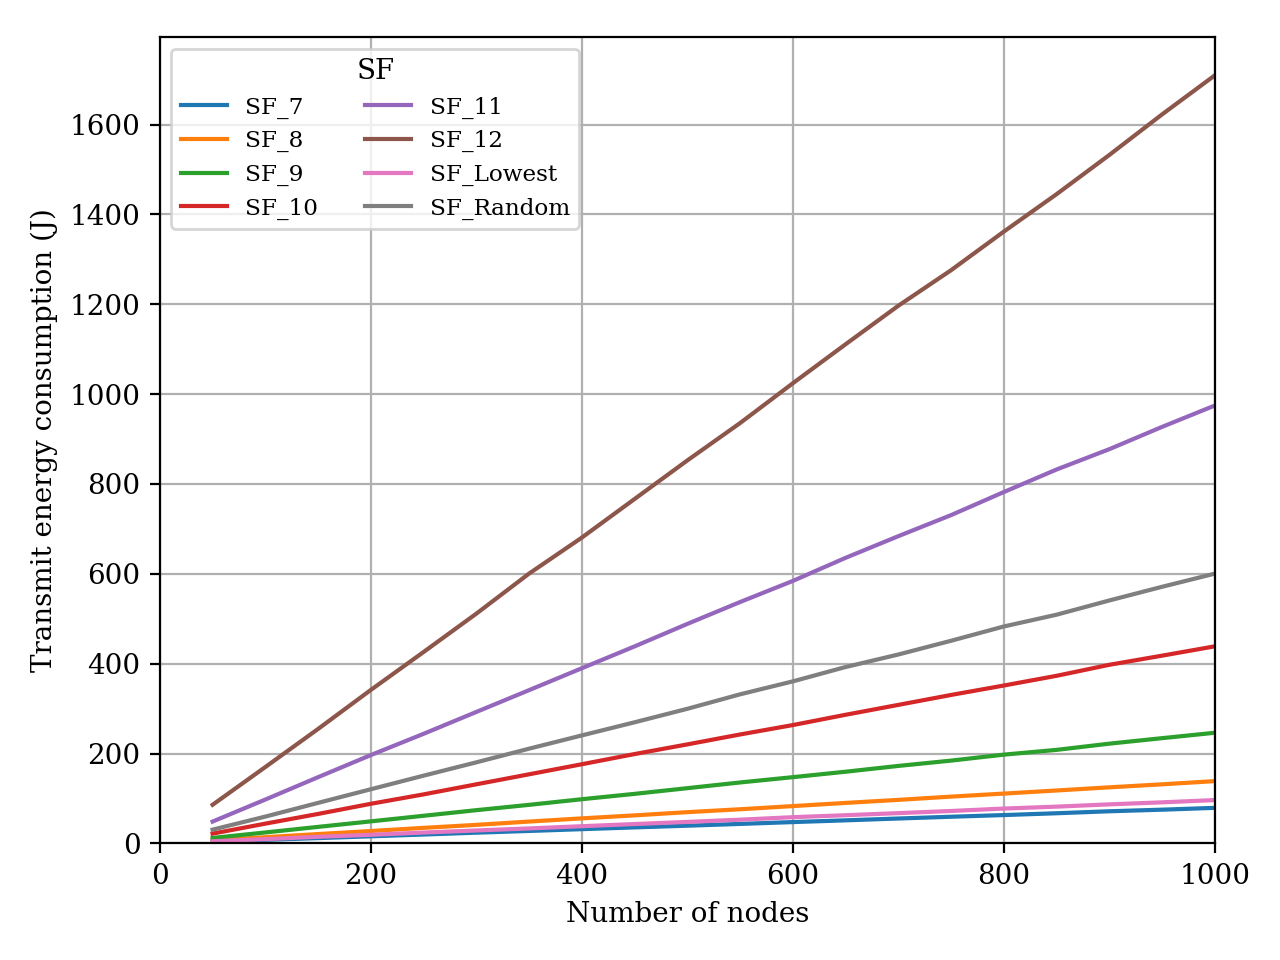
\includegraphics[width=.43\linewidth]{{fig/appendix/sf_energy_r5000_g1_p0.01_s3600}.png}}
\caption{(r = 5000 m, GW = 1)}
\label{fig:sf_r5000_g1}
\end{figure}

\begin{figure}[h]
\centering
\subfigure[PDR]{
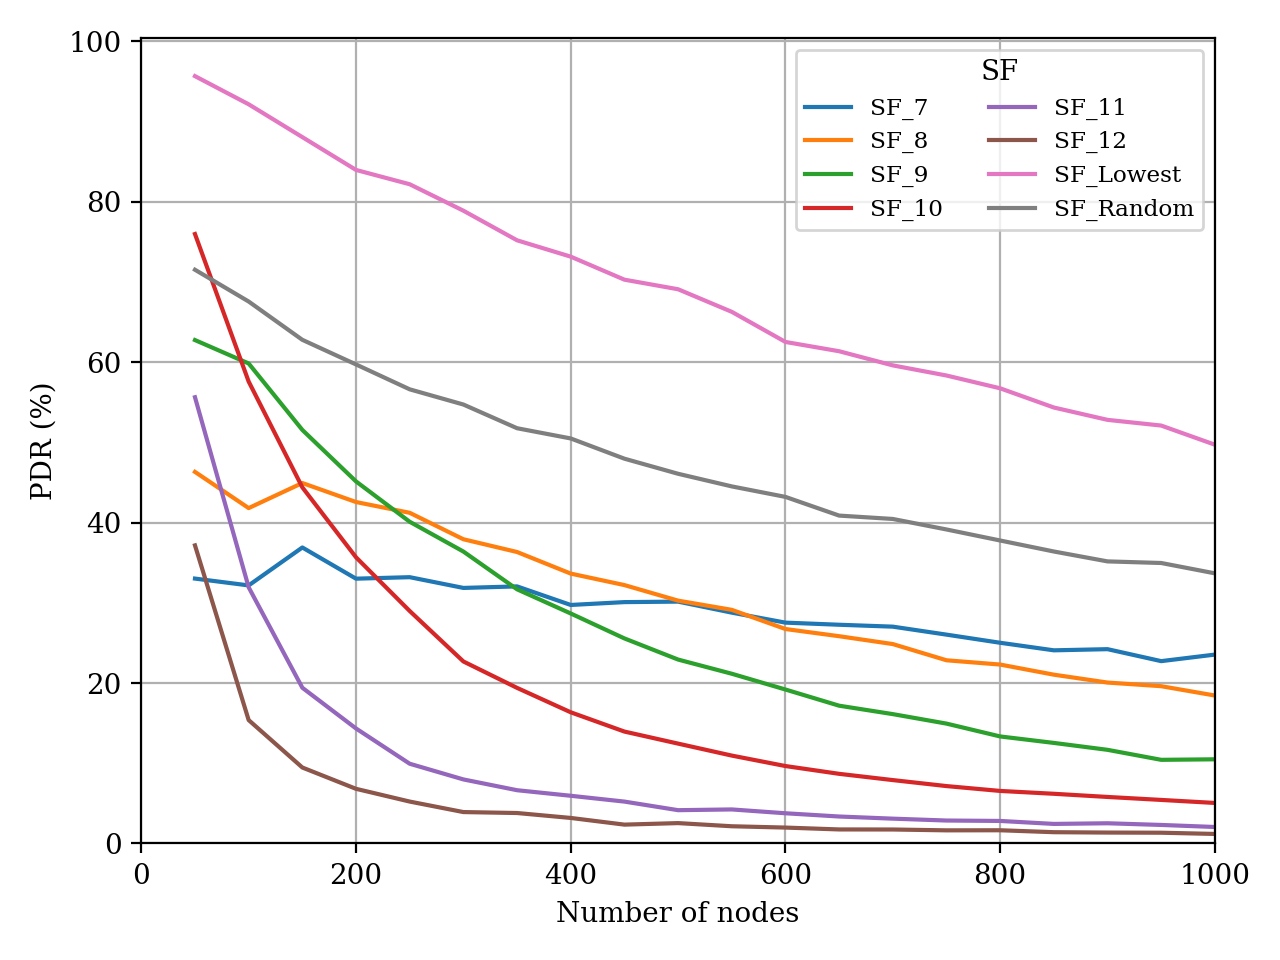
\includegraphics[width=.43\linewidth]{{fig/appendix/sf_pdr_r7000_g1_p0.01_s3600}.png}}
\subfigure[Transmit energy]{
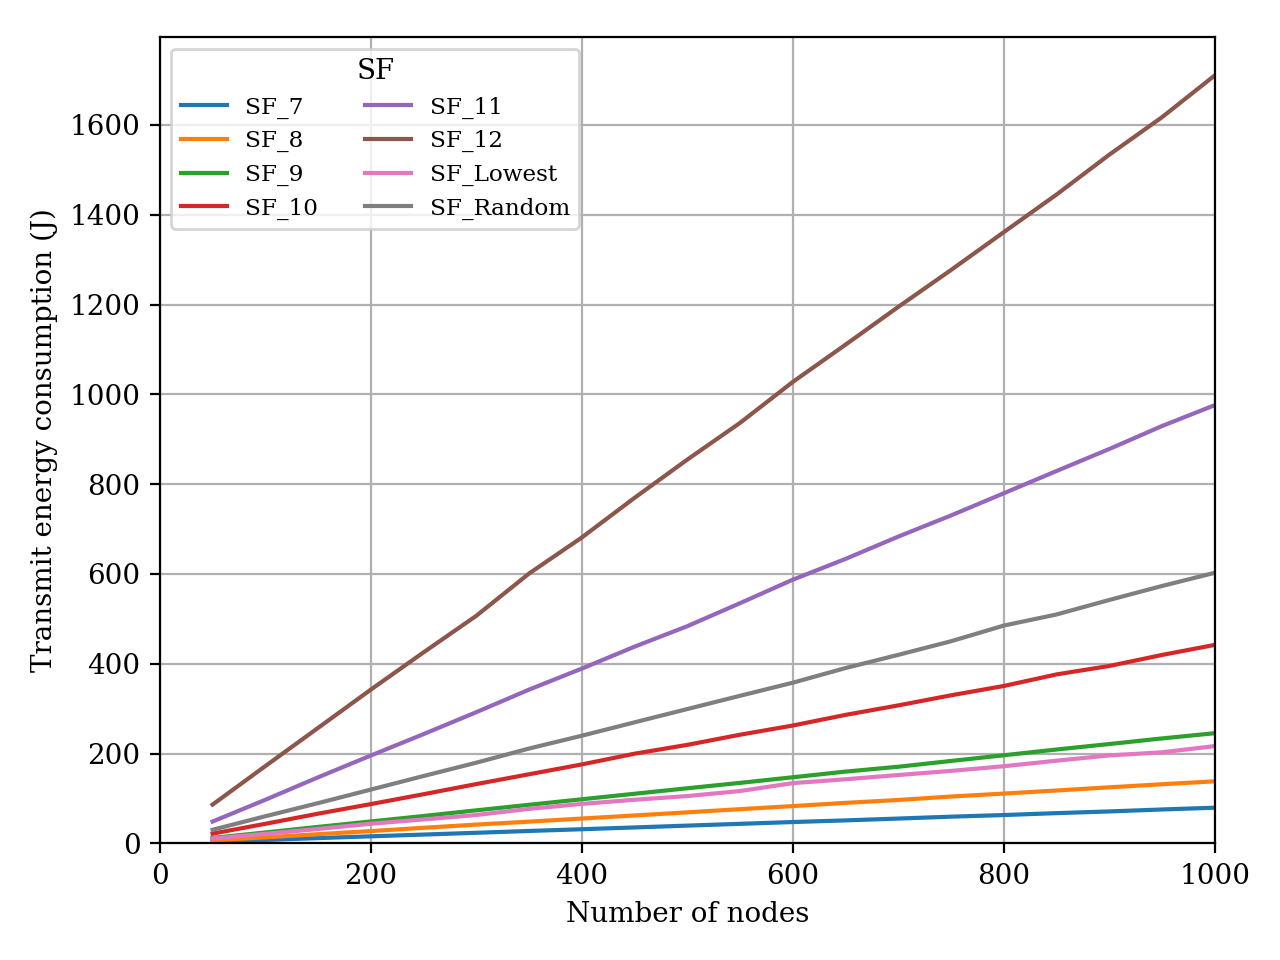
\includegraphics[width=.43\linewidth]{{fig/appendix/sf_energy_r7000_g1_p0.01_s3600}.png}}
\caption{(r = 7000 m, GW = 1)}
\label{fig:sf_r7000_g1}
\end{figure}

\begin{figure}[h]
\centering
\subfigure[PDR]{
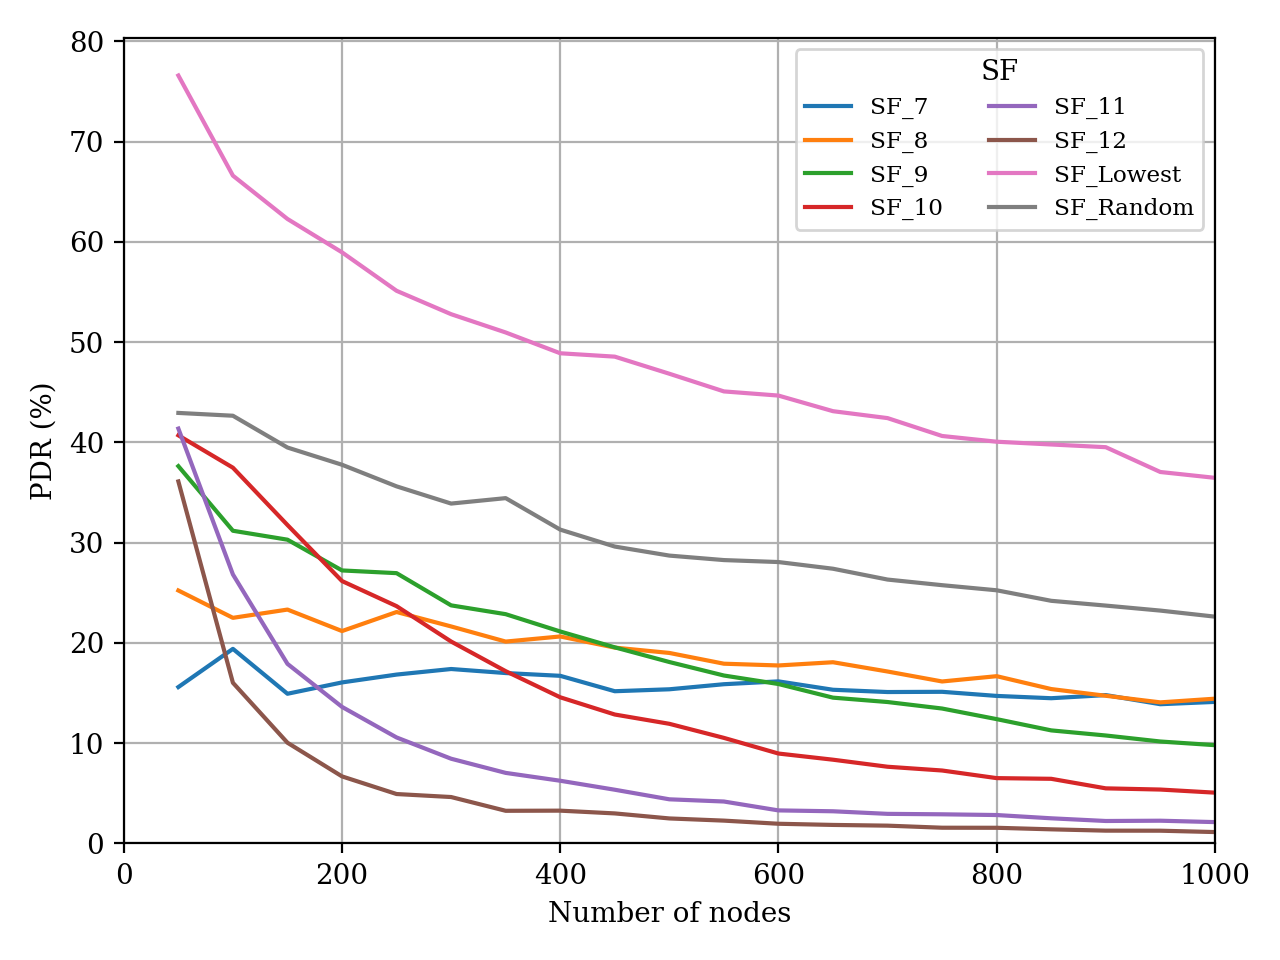
\includegraphics[width=.45\linewidth]{{fig/appendix/sf_pdr_r10000_g1_p0.01_s3600}.png}}
\subfigure[Transmit energy]{
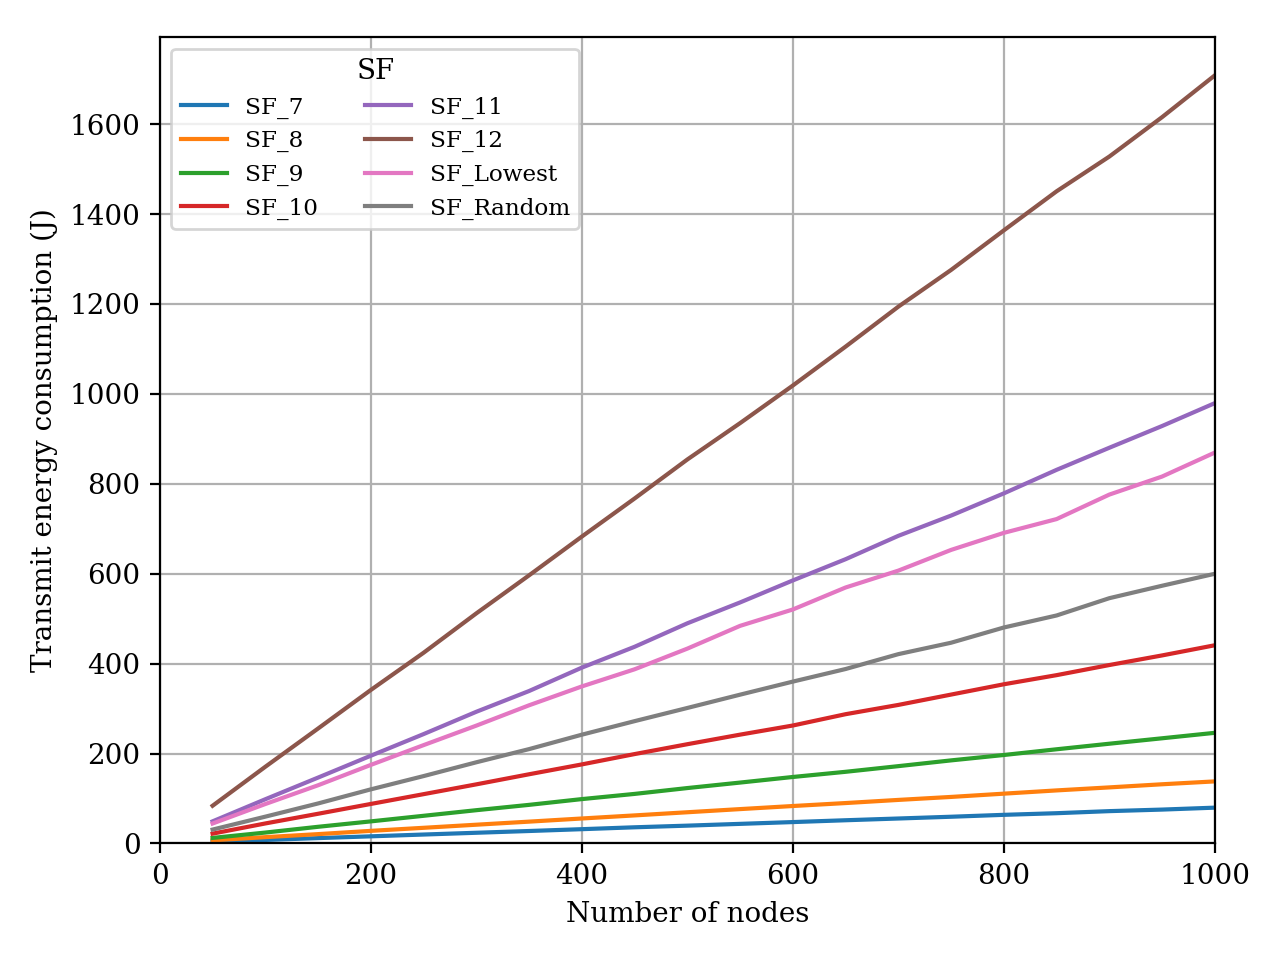
\includegraphics[width=.45\linewidth]{{fig/appendix/sf_energy_r10000_g1_p0.01_s3600}.png}}
\caption{(r = 10000 m, GW = 1)}
\label{fig:sf_r10000_g1}
\end{figure}


\begin{figure}[h]
\centering
\subfigure[PDR]{
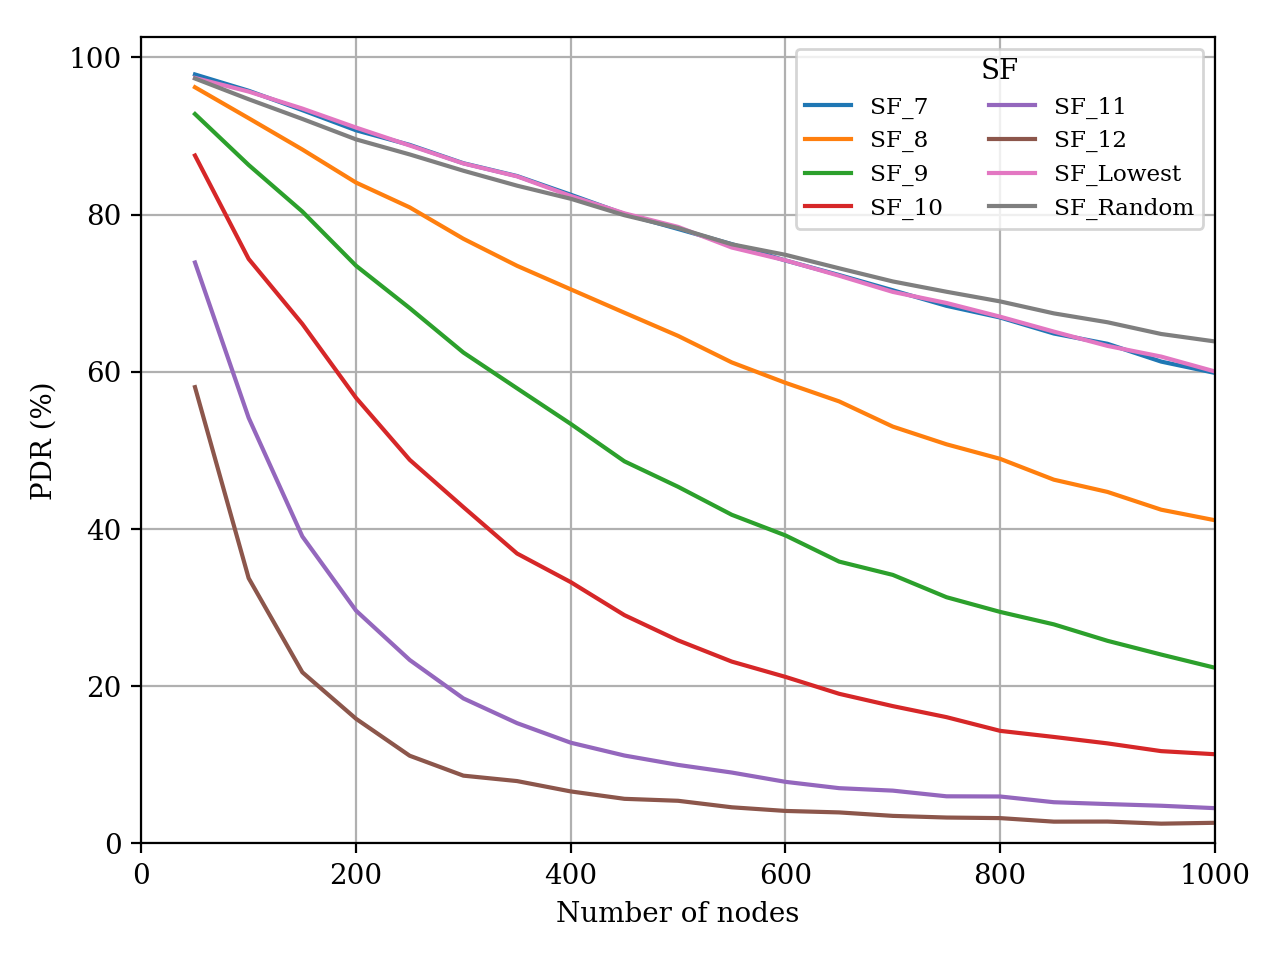
\includegraphics[width=.45\linewidth]{{fig/appendix/sf_pdr_r3000_g2_p0.01_s3600}.png}}
\subfigure[Transmit energy]{
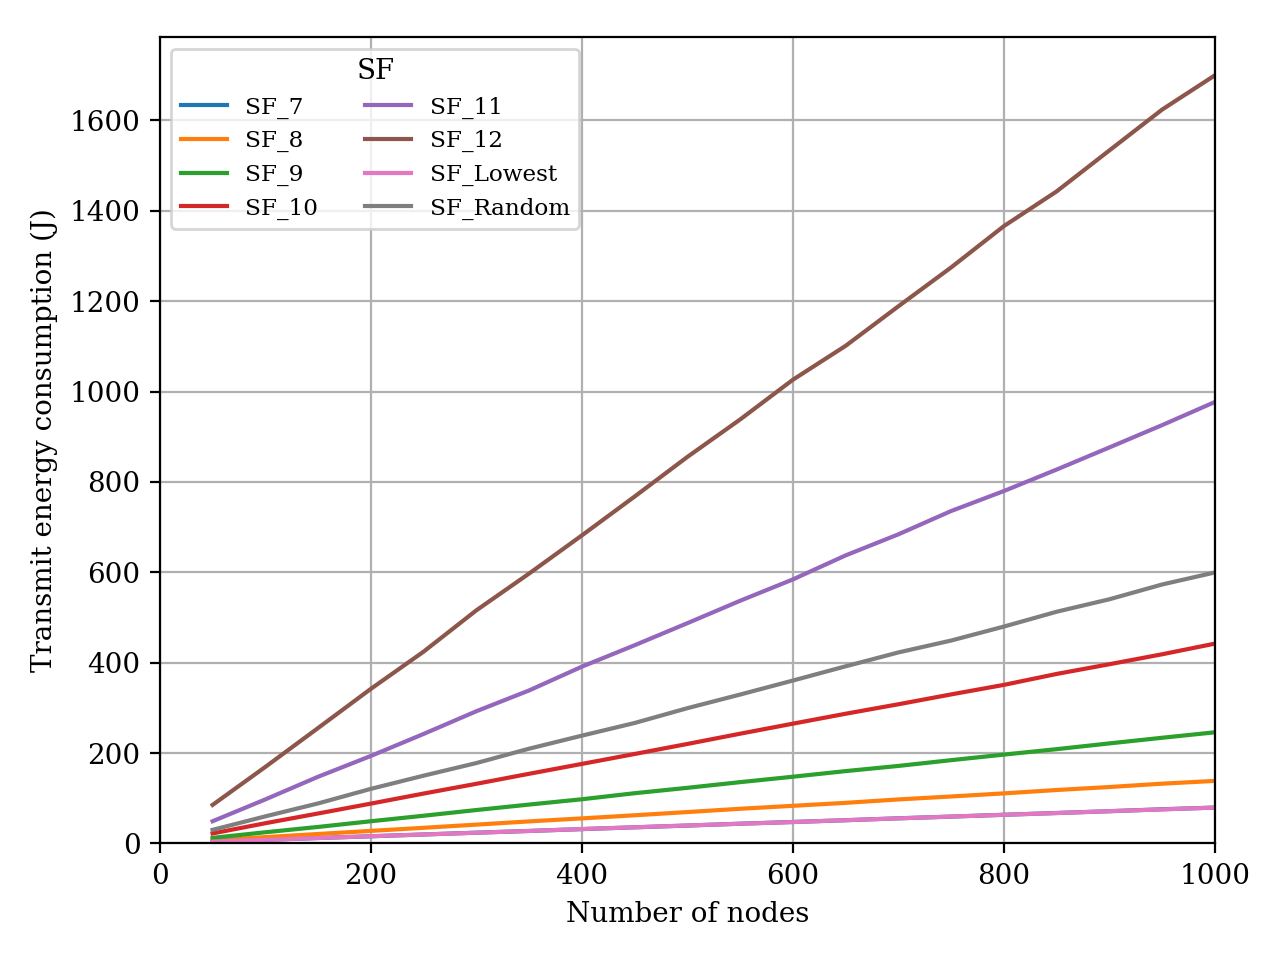
\includegraphics[width=.45\linewidth]{{fig/appendix/sf_energy_r3000_g2_p0.01_s3600}.png}}
\caption{(r = 3000 m, GW = 2)}
\label{fig:sf_r3000_g2}
\end{figure}

\begin{figure}[h]
\centering
\subfigure[PDR]{
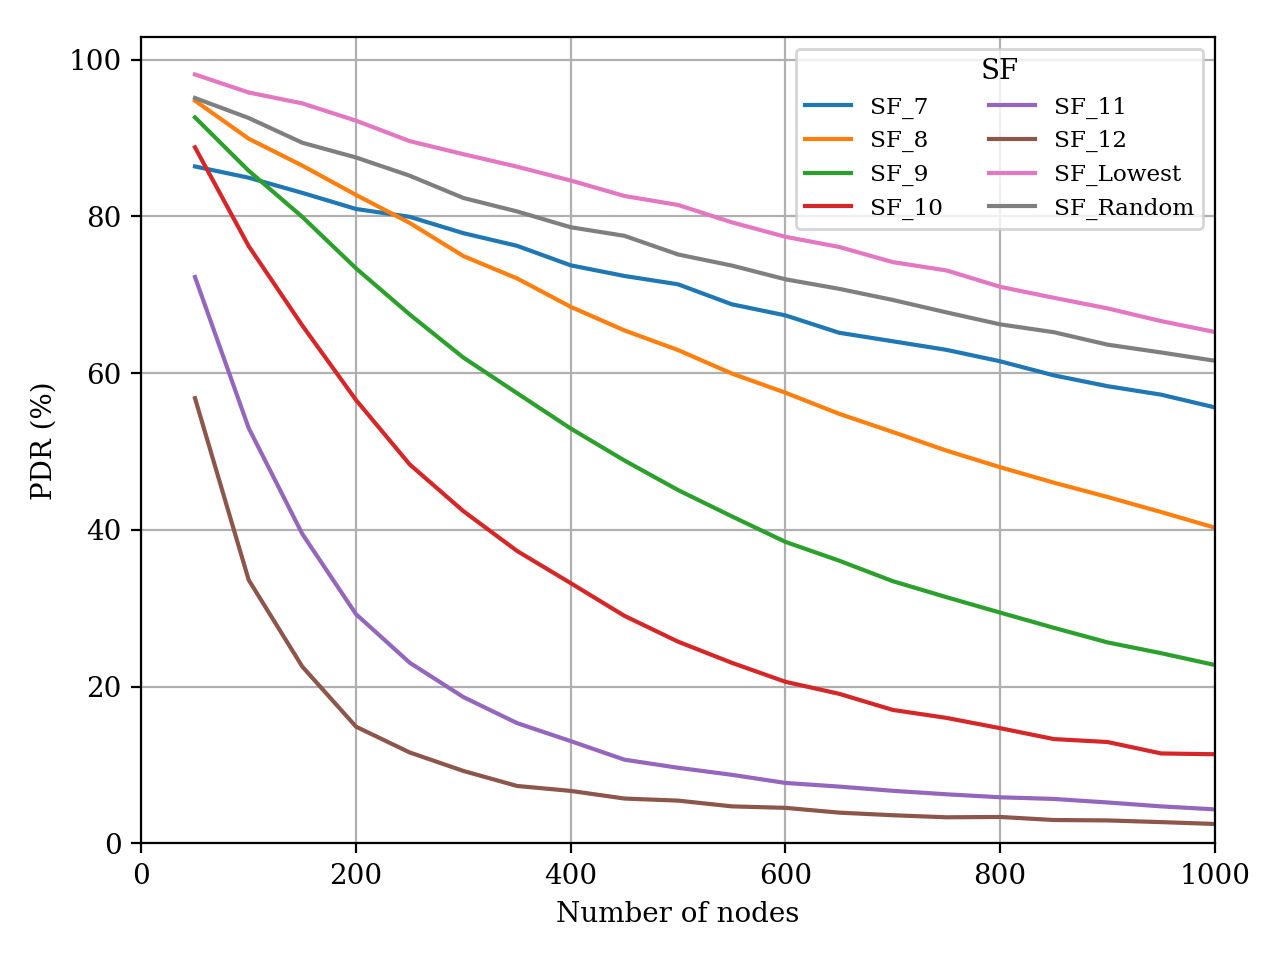
\includegraphics[width=.45\linewidth]{{fig/appendix/sf_pdr_r5000_g2_p0.01_s3600}.png}}
\subfigure[Transmit energy]{
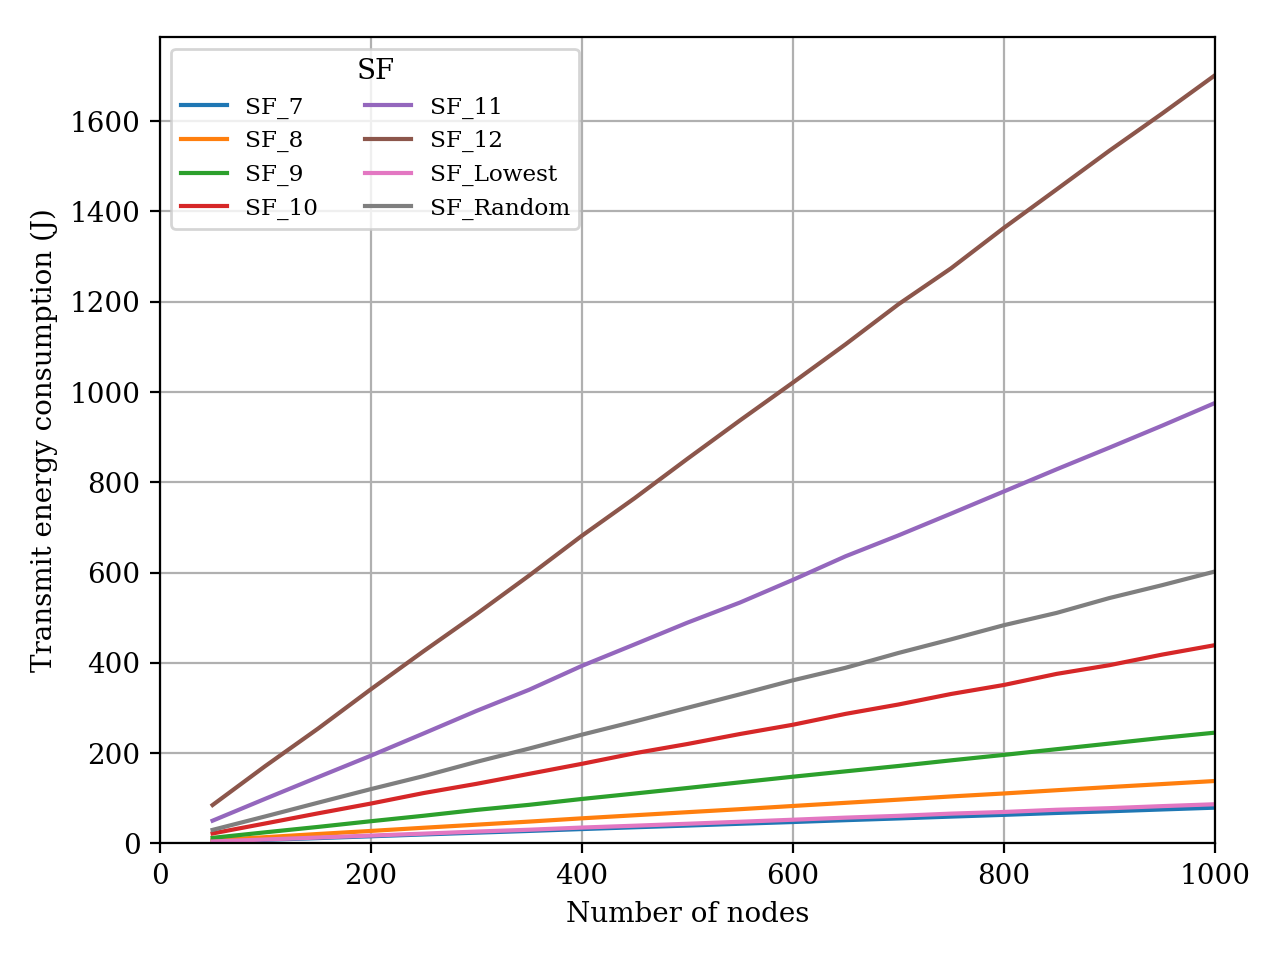
\includegraphics[width=.45\linewidth]{{fig/appendix/sf_energy_r5000_g2_p0.01_s3600}.png}}
\caption{(r = 5000 m, GW = 2)}
\label{fig:sf_r5000_g2}
\end{figure}

\begin{figure}[h]
\centering
\subfigure[PDR]{
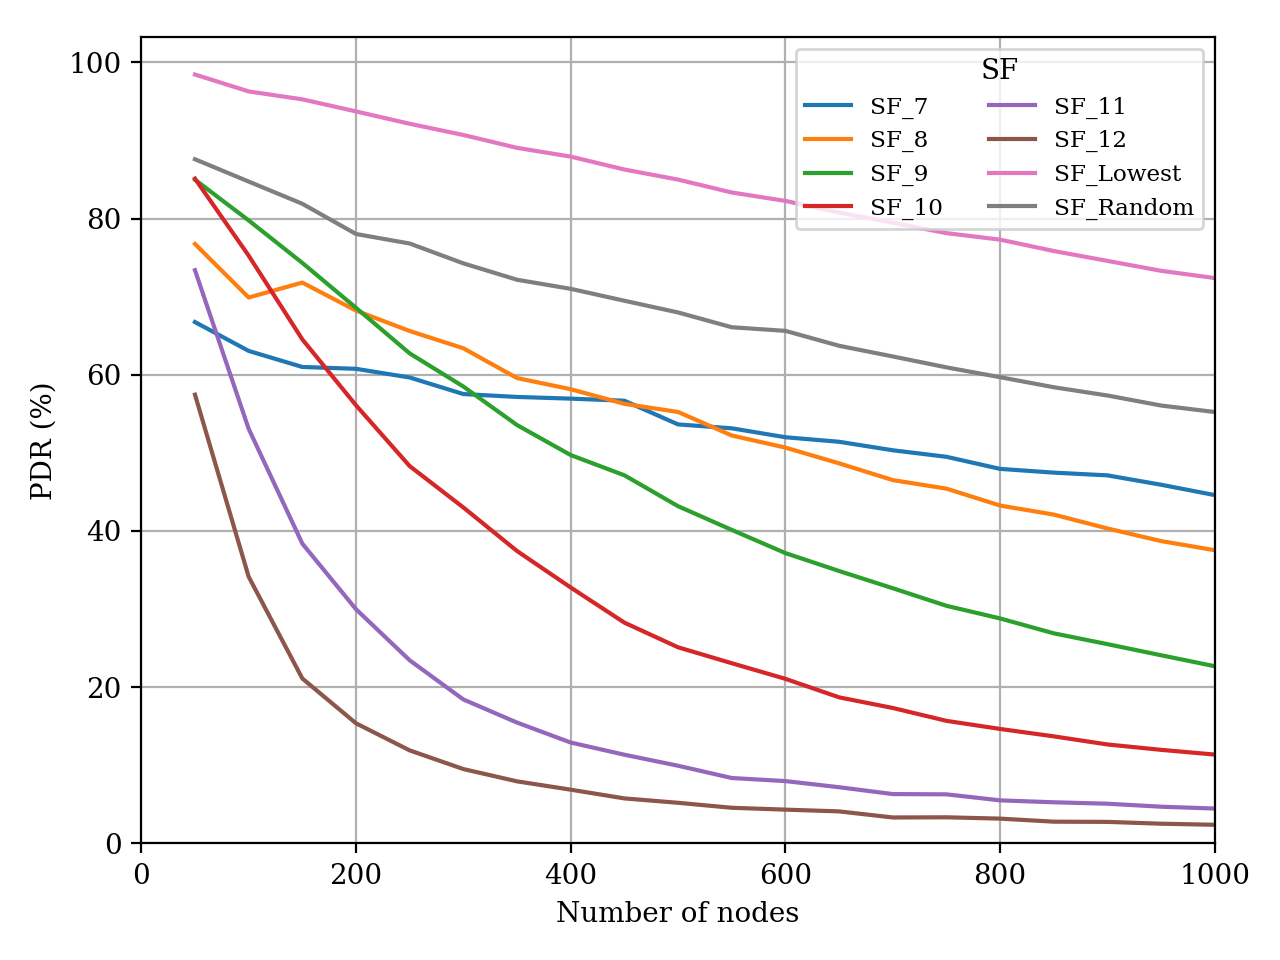
\includegraphics[width=.45\linewidth]{{fig/appendix/sf_pdr_r7000_g2_p0.01_s3600}.png}}
\subfigure[Transmit energy]{
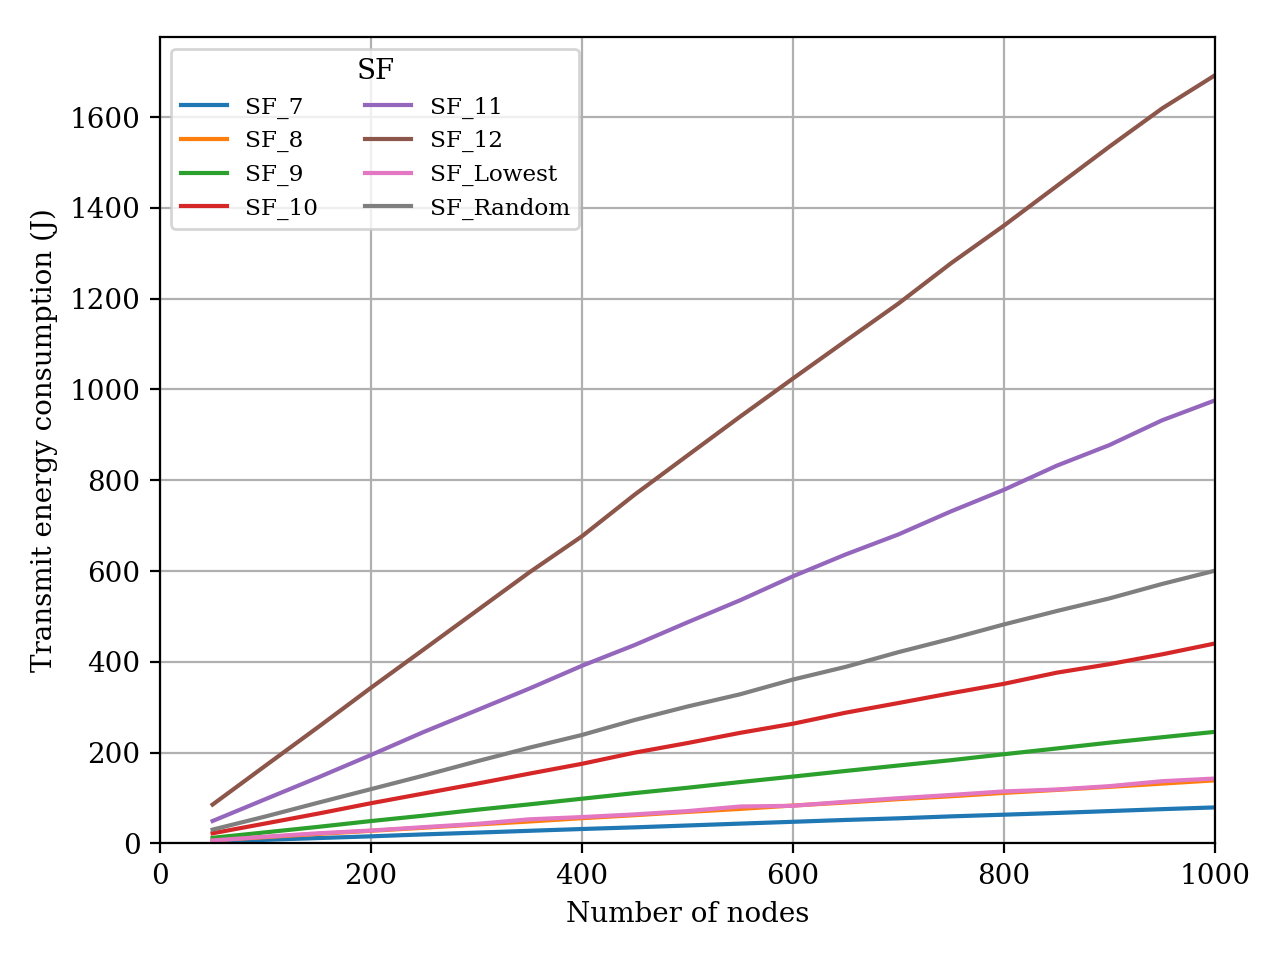
\includegraphics[width=.45\linewidth]{{fig/appendix/sf_energy_r7000_g2_p0.01_s3600}.png}}
\caption{(r = 7000 m, GW = 2)}
\label{fig:sf_r7000_g2}
\end{figure}

\begin{figure}[h]
\centering
\subfigure[PDR]{
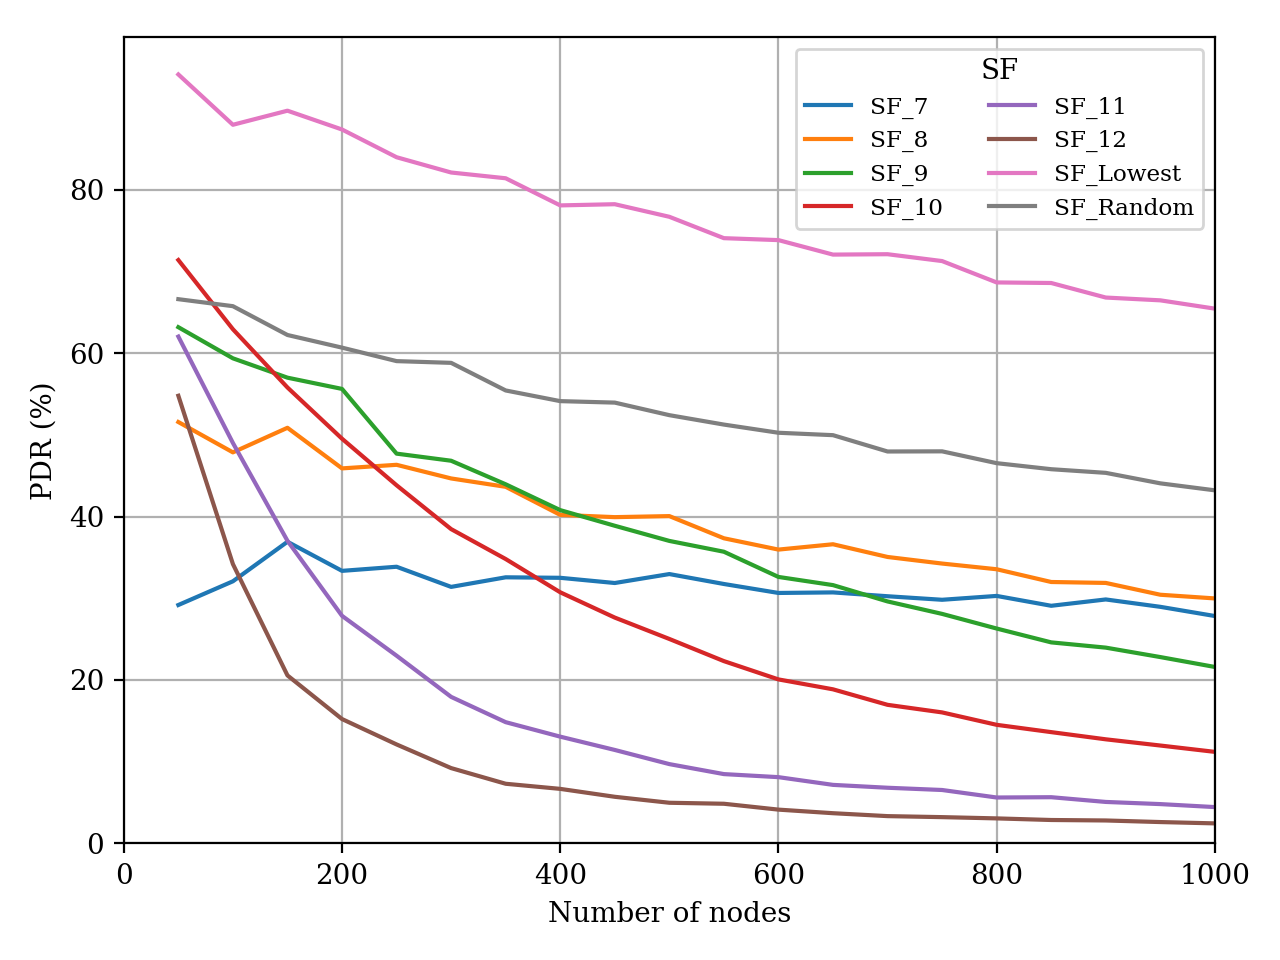
\includegraphics[width=.45\linewidth]{{fig/appendix/sf_pdr_r10000_g2_p0.01_s3600}.png}}
\subfigure[Transmit energy]{
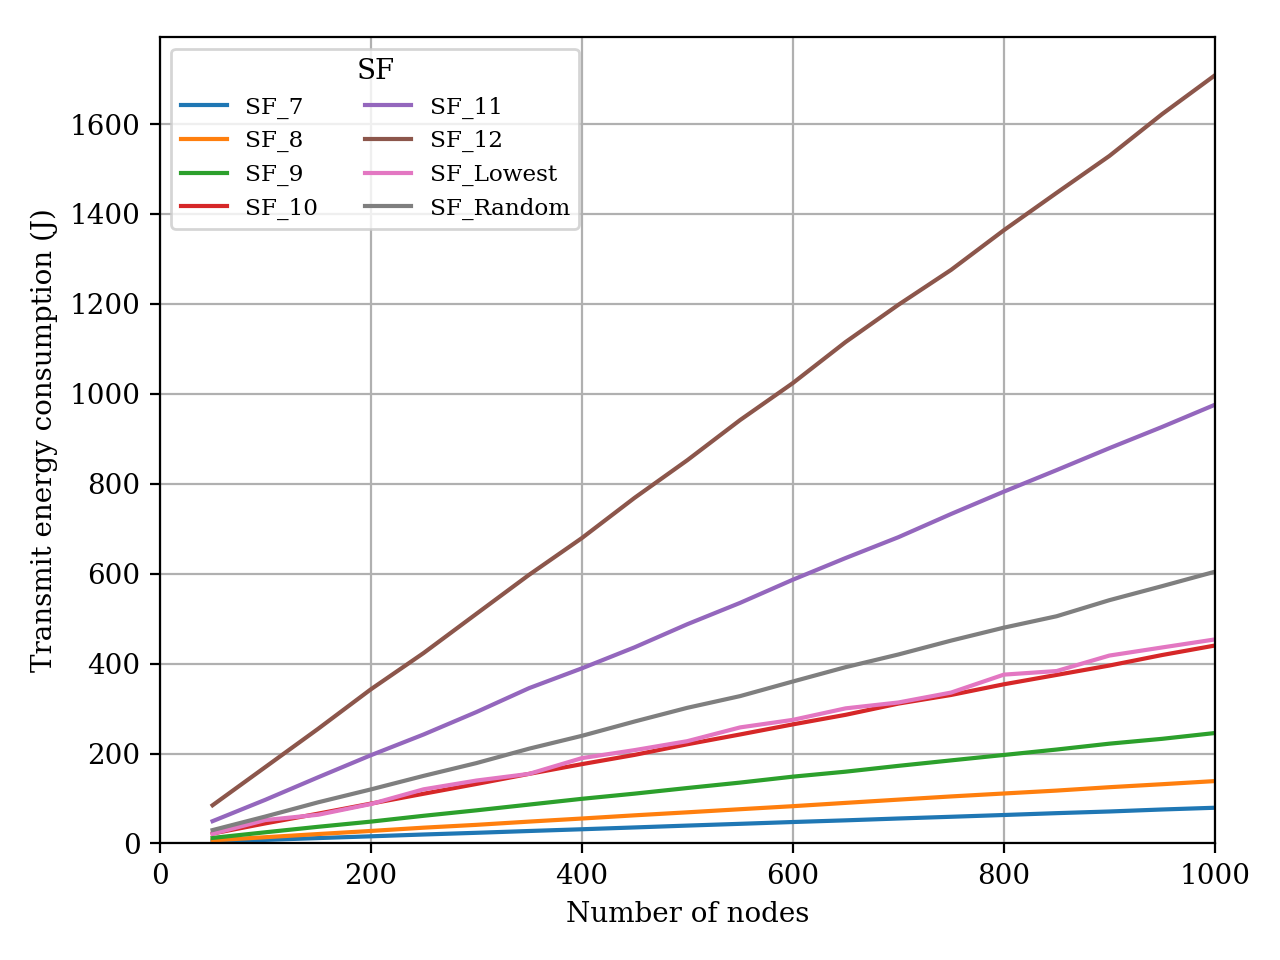
\includegraphics[width=.45\linewidth]{{fig/appendix/sf_energy_r10000_g2_p0.01_s3600}.png}}
\caption{(r = 10000 m, GW = 2)}
\label{fig:sf_r10000_g2}
\end{figure}


\begin{figure}[h]
\centering
\subfigure[PDR]{
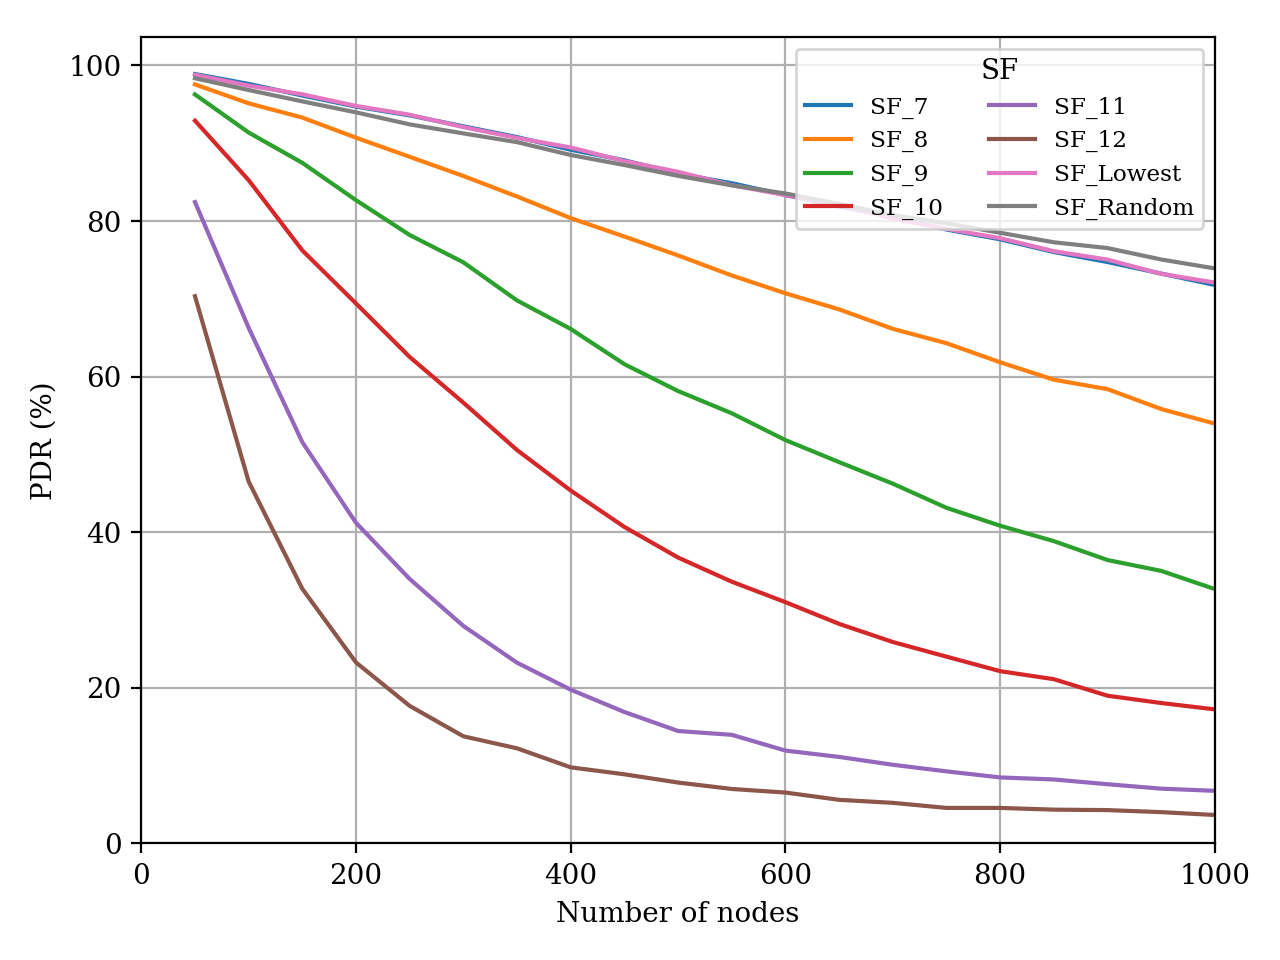
\includegraphics[width=.45\linewidth]{{fig/appendix/sf_pdr_r3000_g3_p0.01_s3600}.png}}
\subfigure[Transmit energy]{
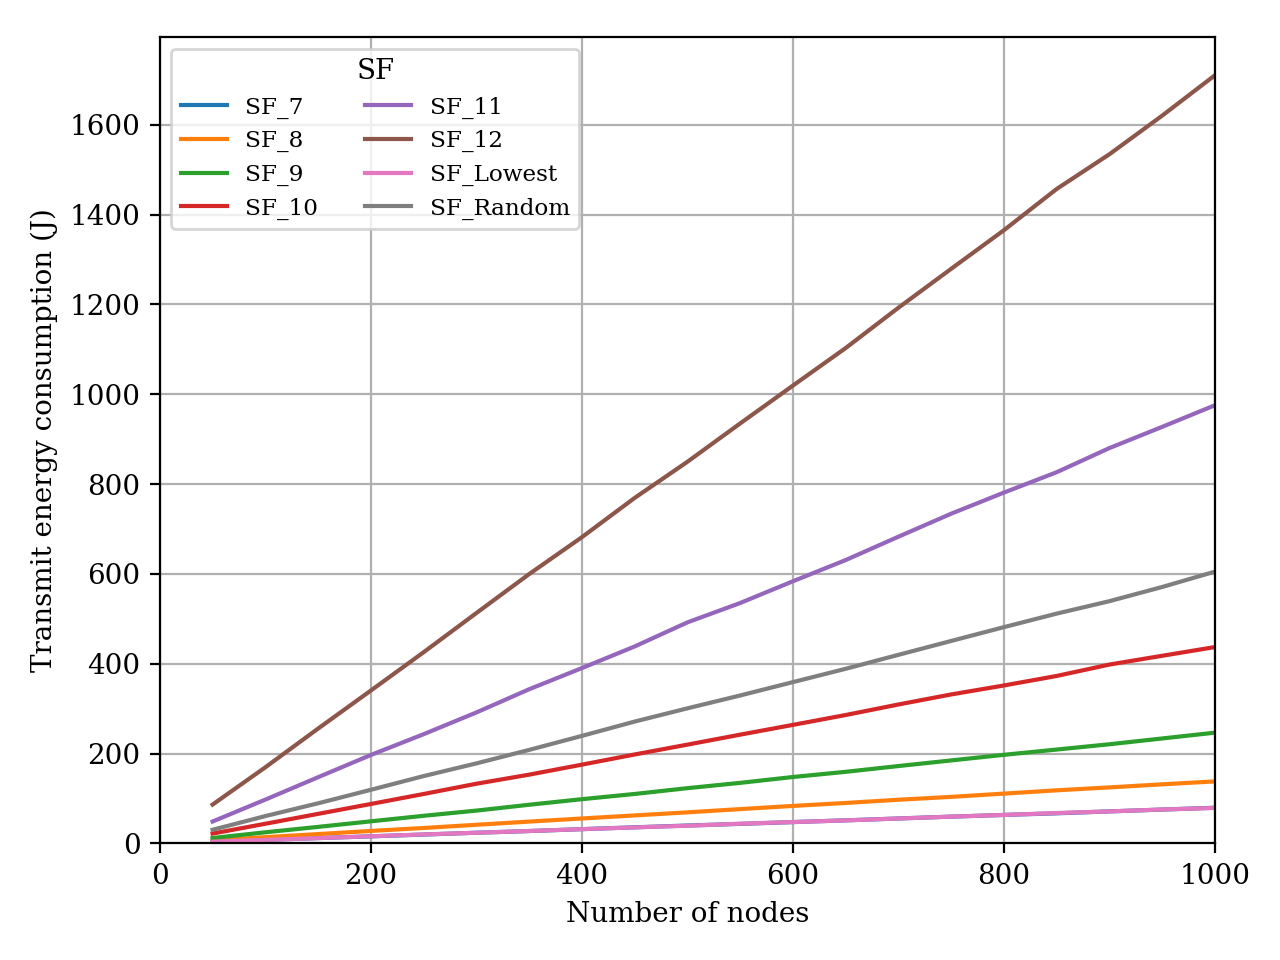
\includegraphics[width=.45\linewidth]{{fig/appendix/sf_energy_r3000_g3_p0.01_s3600}.png}}
\caption{(r = 3000 m, GW = 3)}
\label{fig:sf_r3000_g3}
\end{figure}

\begin{figure}[h]
\centering
\subfigure[PDR]{
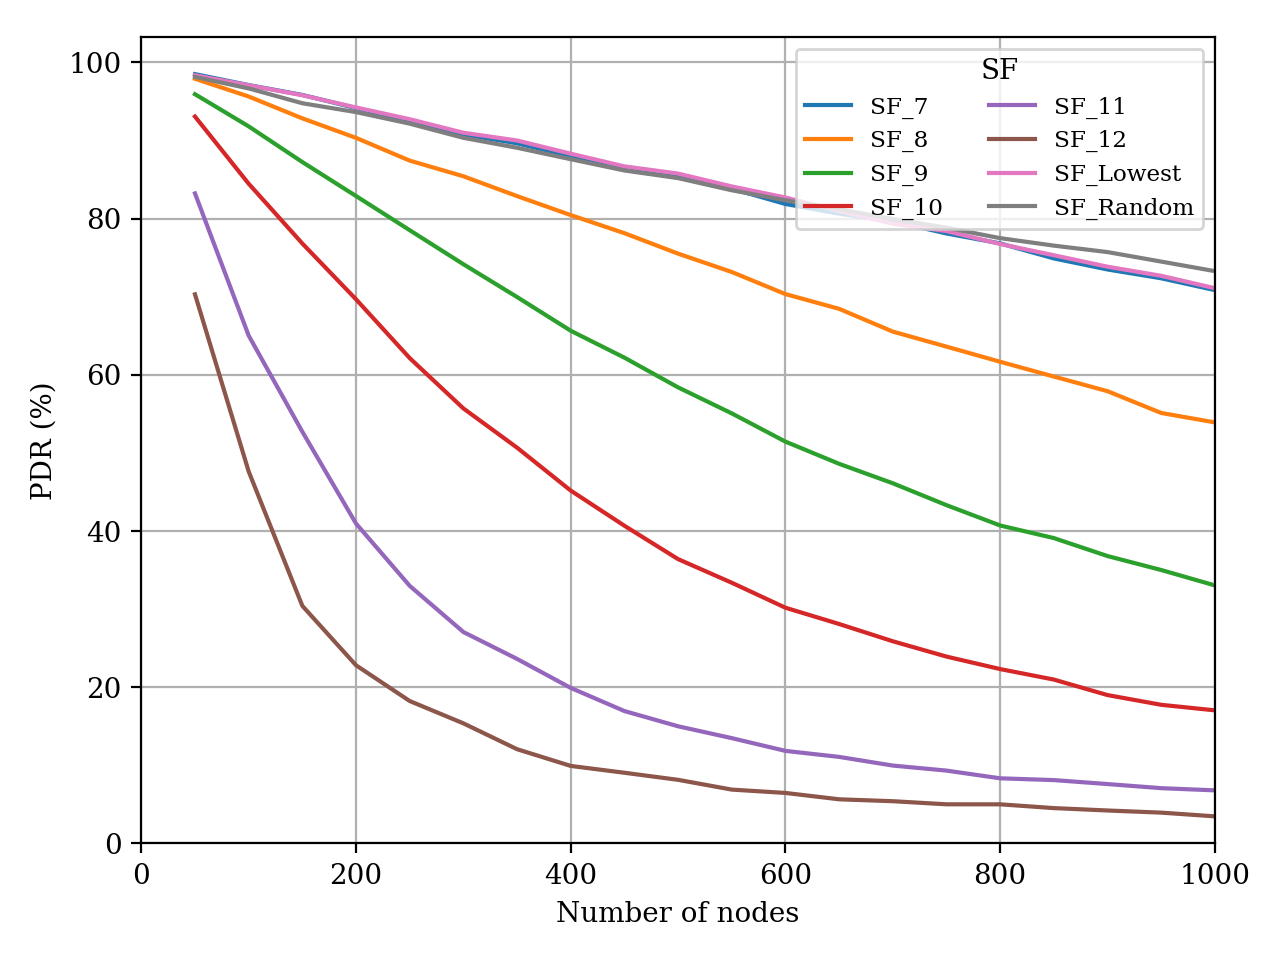
\includegraphics[width=.45\linewidth]{{fig/appendix/sf_pdr_r5000_g3_p0.01_s3600}.png}}
\subfigure[Transmit energy]{
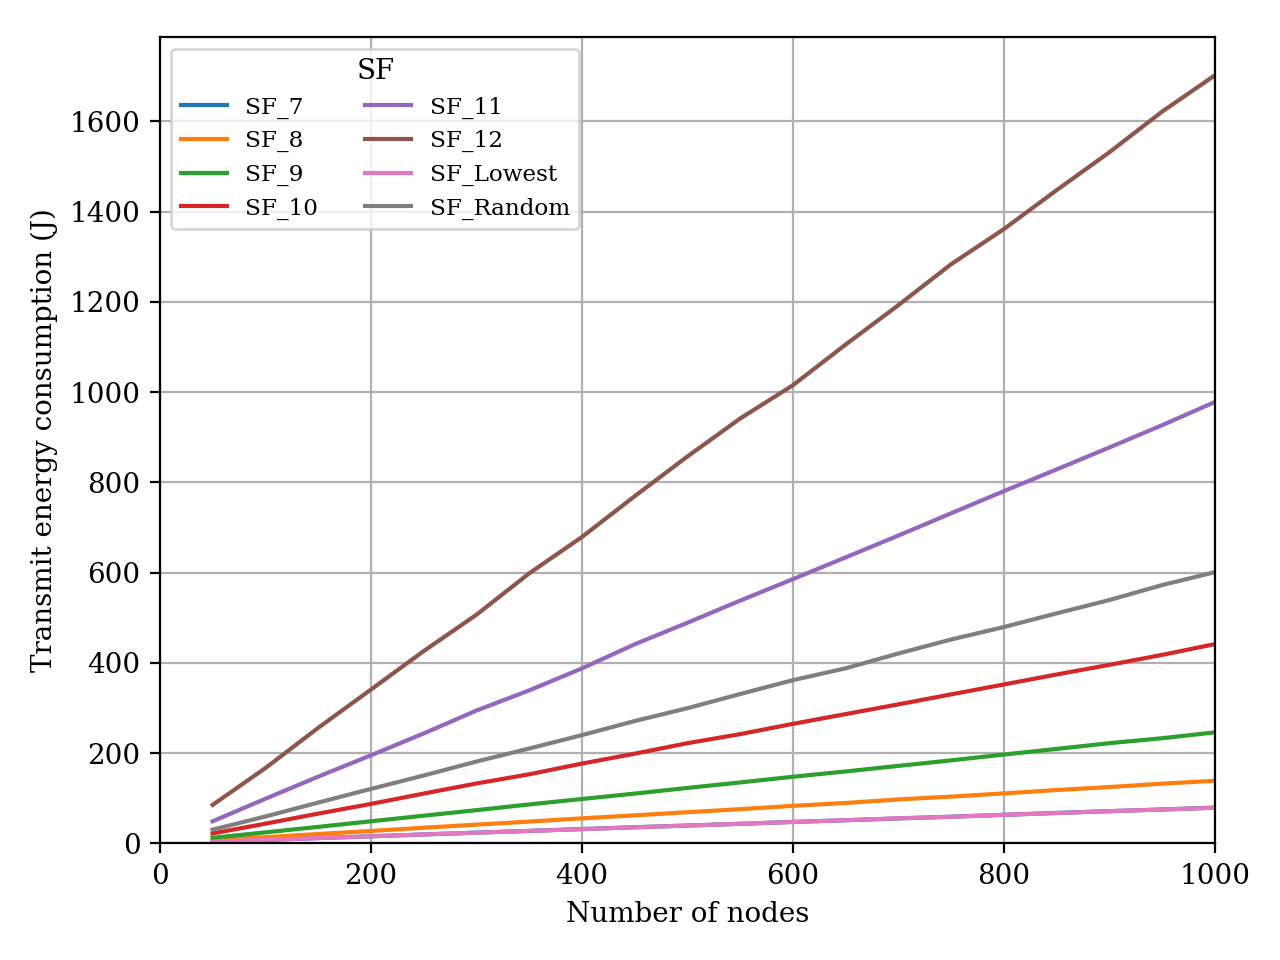
\includegraphics[width=.45\linewidth]{{fig/appendix/sf_energy_r5000_g3_p0.01_s3600}.png}}
\caption{(r = 5000 m, GW = 3)}
\label{fig:sf_r5000_g3}
\end{figure}

\begin{figure}[h]
\centering
\subfigure[PDR]{
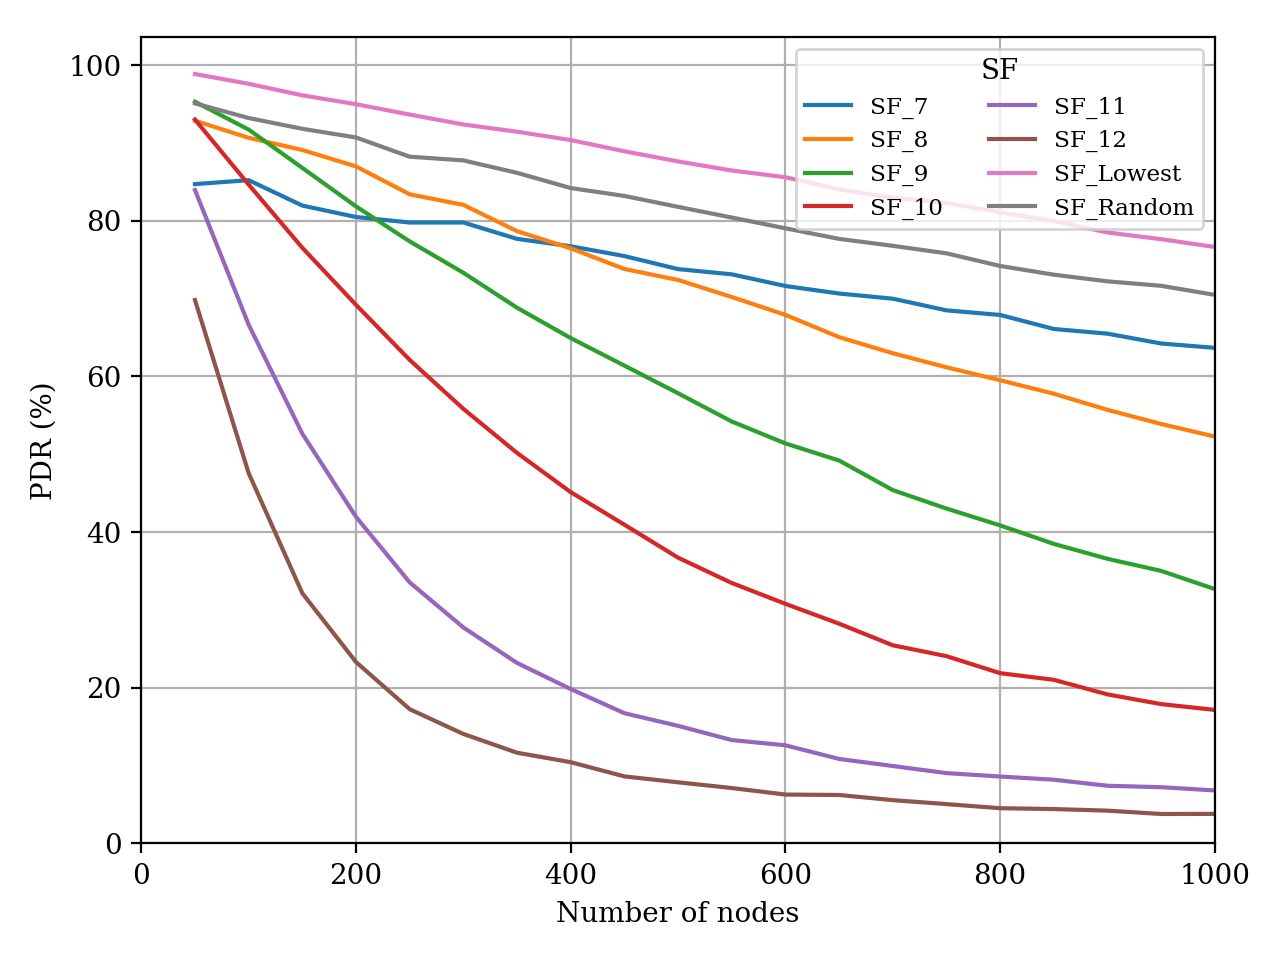
\includegraphics[width=.45\linewidth]{{fig/appendix/sf_pdr_r7000_g3_p0.01_s3600}.png}}
\subfigure[Transmit energy]{
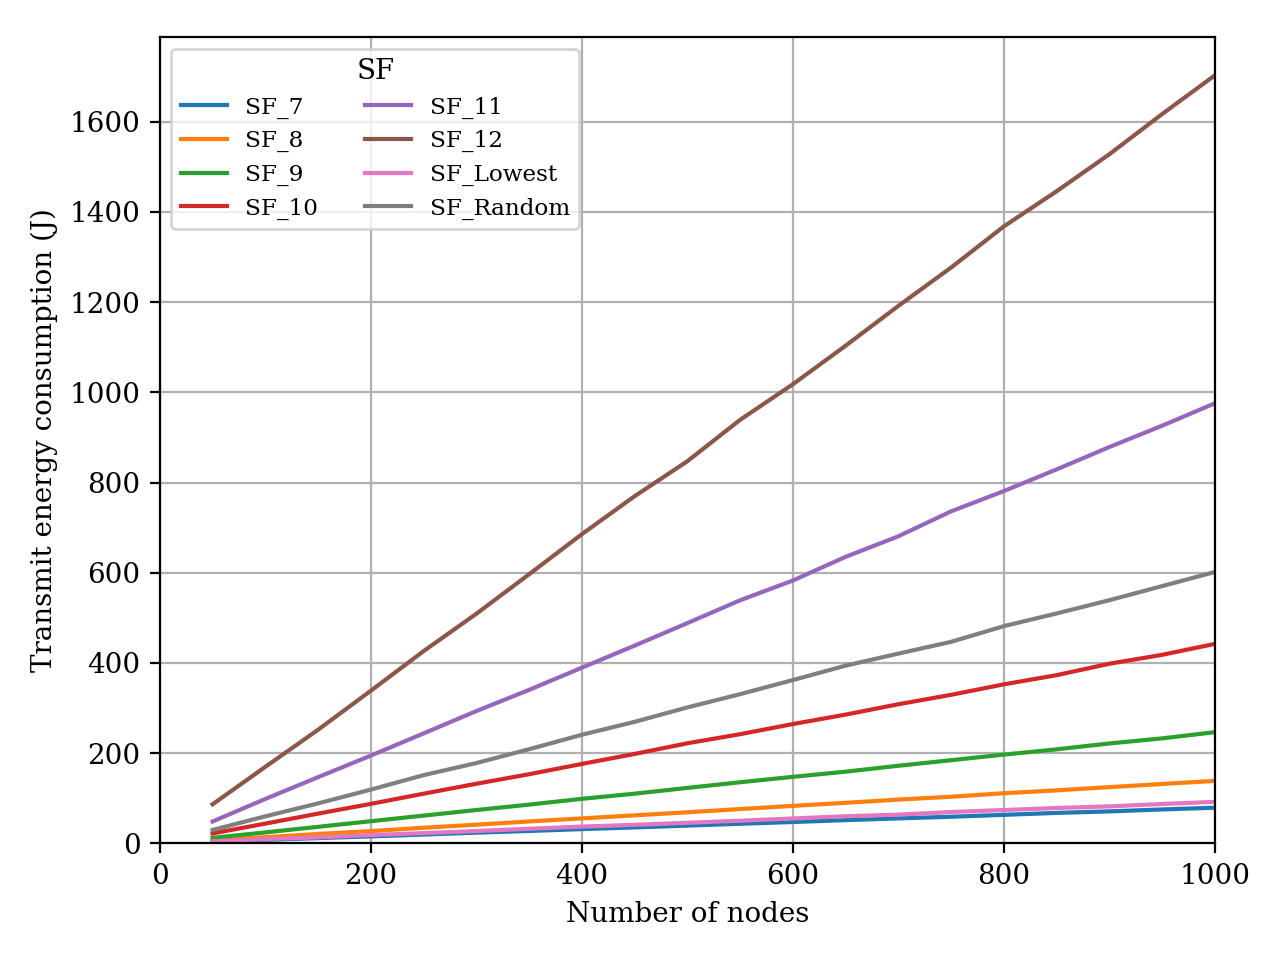
\includegraphics[width=.45\linewidth]{{fig/appendix/sf_energy_r7000_g3_p0.01_s3600}.png}}
\caption{(r = 7000 m, GW = 3)}
\label{fig:sf_r7000_g3}
\end{figure}

\begin{figure}[h]
\centering
\subfigure[PDR]{
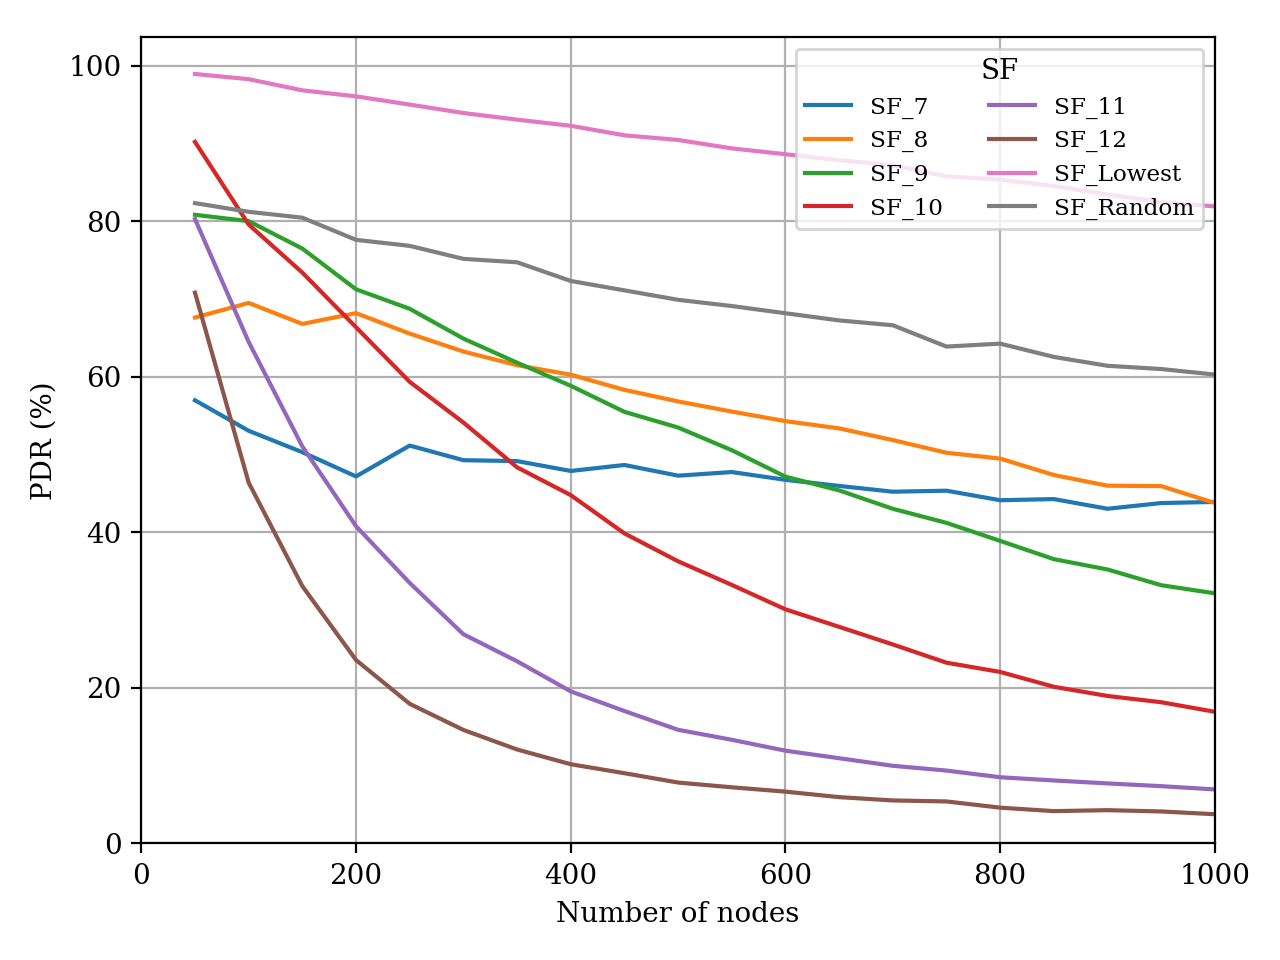
\includegraphics[width=.45\linewidth]{{fig/appendix/sf_pdr_r10000_g3_p0.01_s3600}.png}}
\subfigure[Transmit energy]{
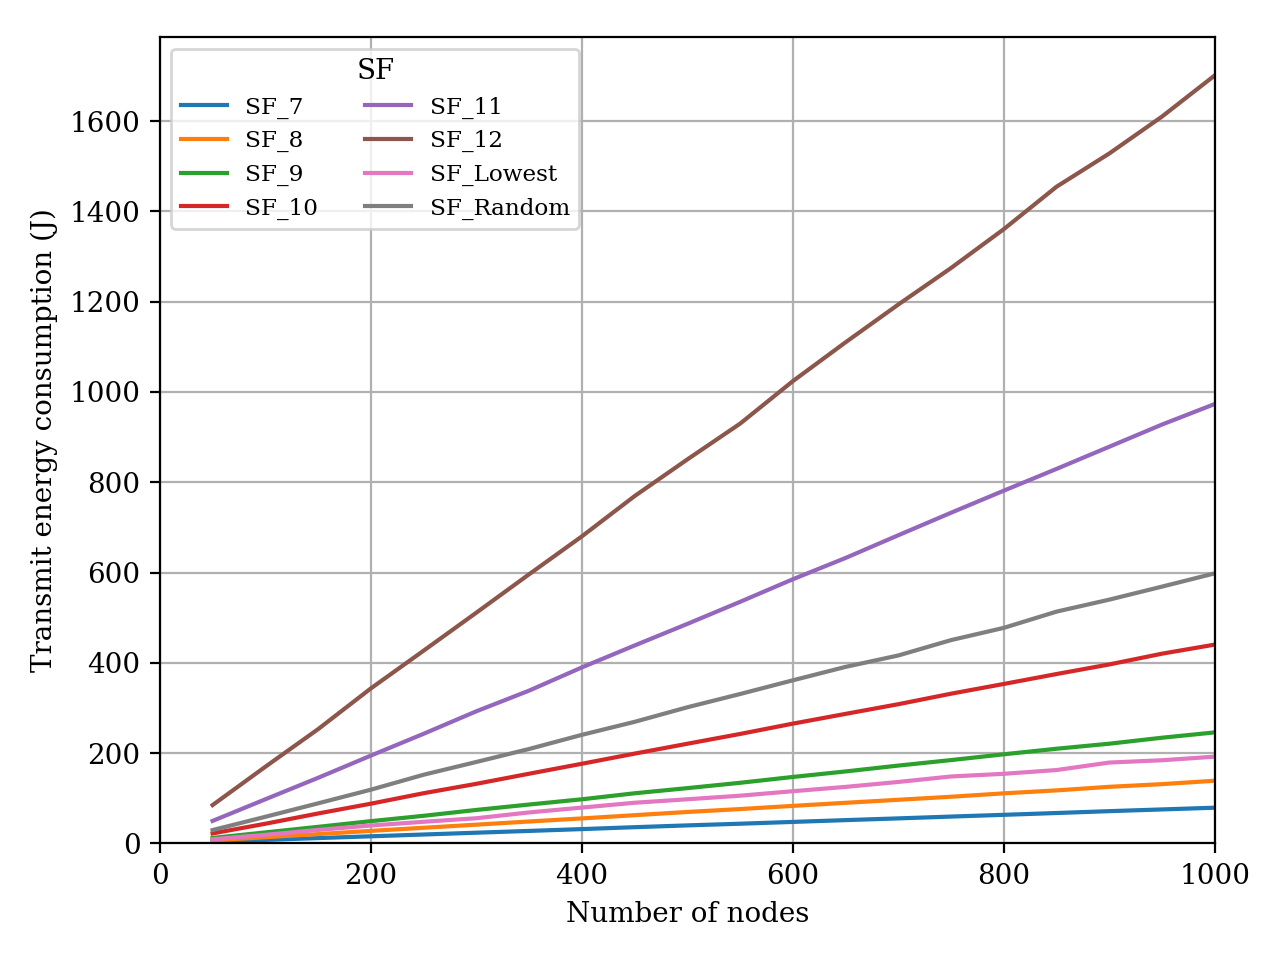
\includegraphics[width=.45\linewidth]{{fig/appendix/sf_energy_r10000_g3_p0.01_s3600}.png}}
\caption{(r = 10000 m, GW = 3)}
\label{fig:sf_r10000_g3}
\end{figure}


\chapter{APPENDIX B}

\begin{figure}[h]
\centering
\subfigure[PDR]{
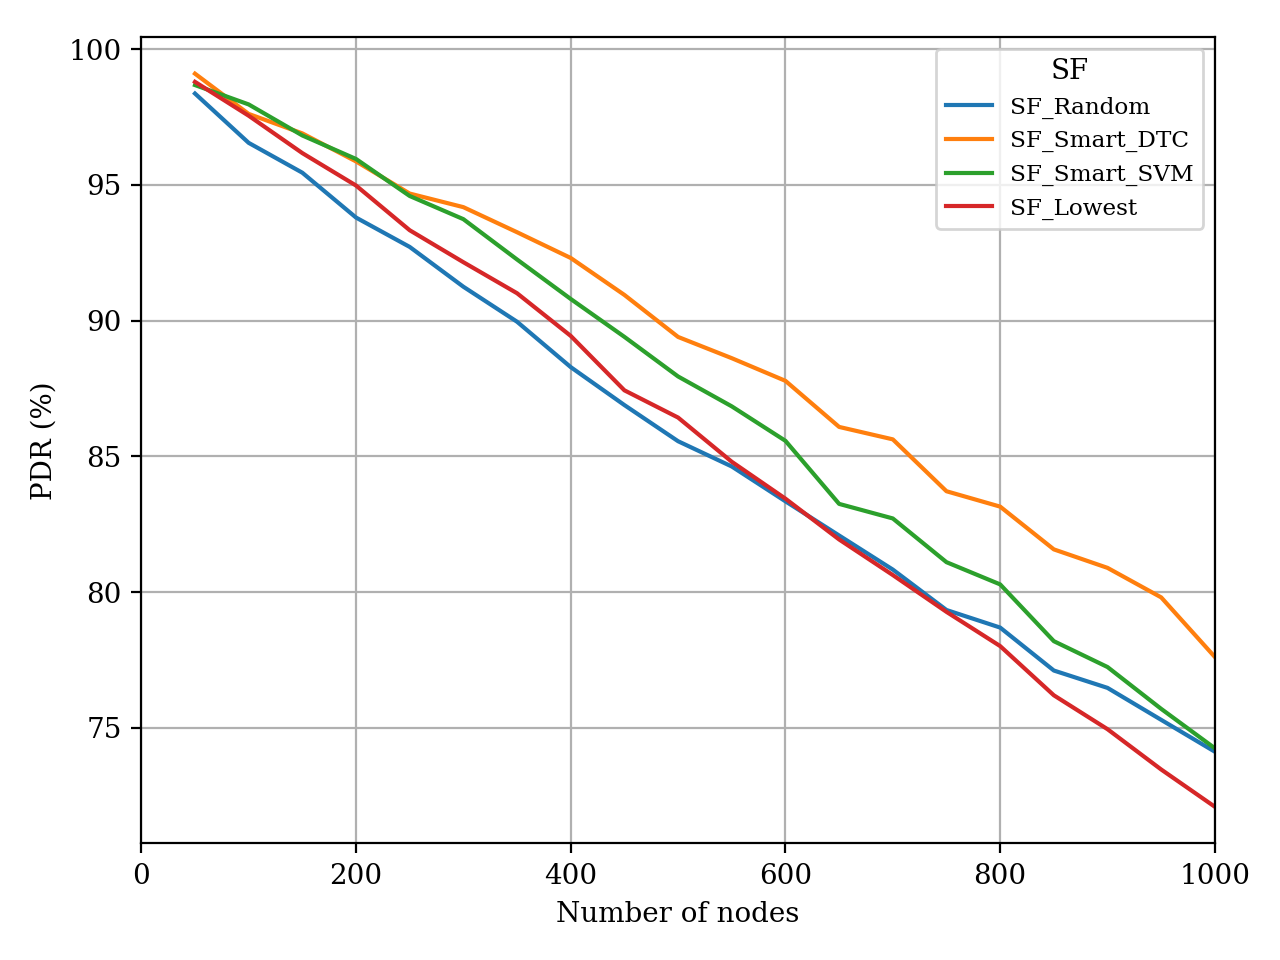
\includegraphics[width=.43\linewidth]{{fig/appendix/prediction_pdr_r3000_g3_p0.01_s3600}.png}}
\subfigure[Transmit energy]{
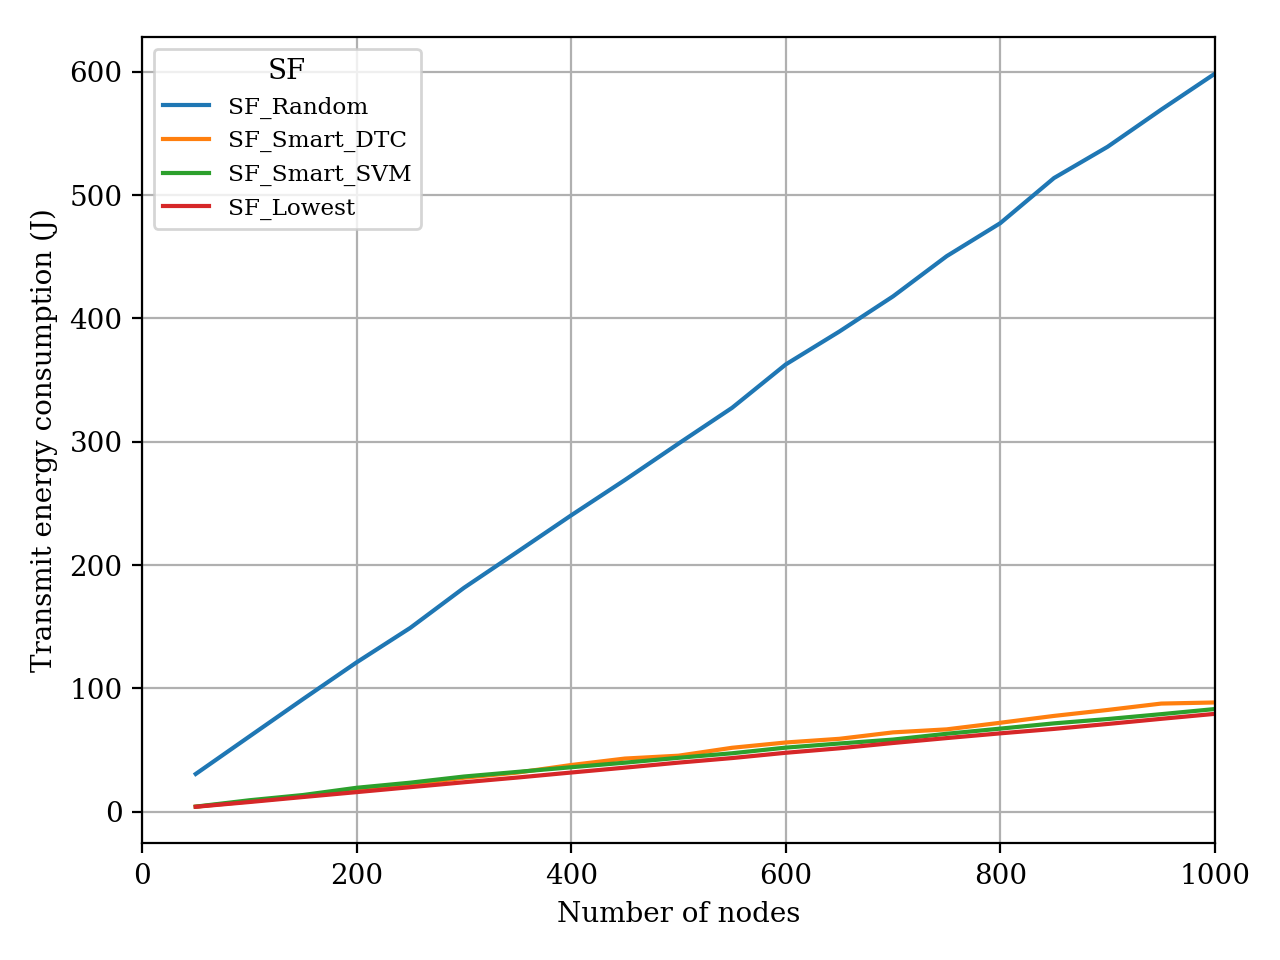
\includegraphics[width=.43\linewidth]{{fig/appendix/prediction_energy_r3000_g3_p0.01_s3600}.png}}
\caption{(r = 3000 m, GW = 3)}
\label{fig:prediction_r3000_g3}
\end{figure}

\begin{figure}[h]
\centering
\subfigure[PDR]{
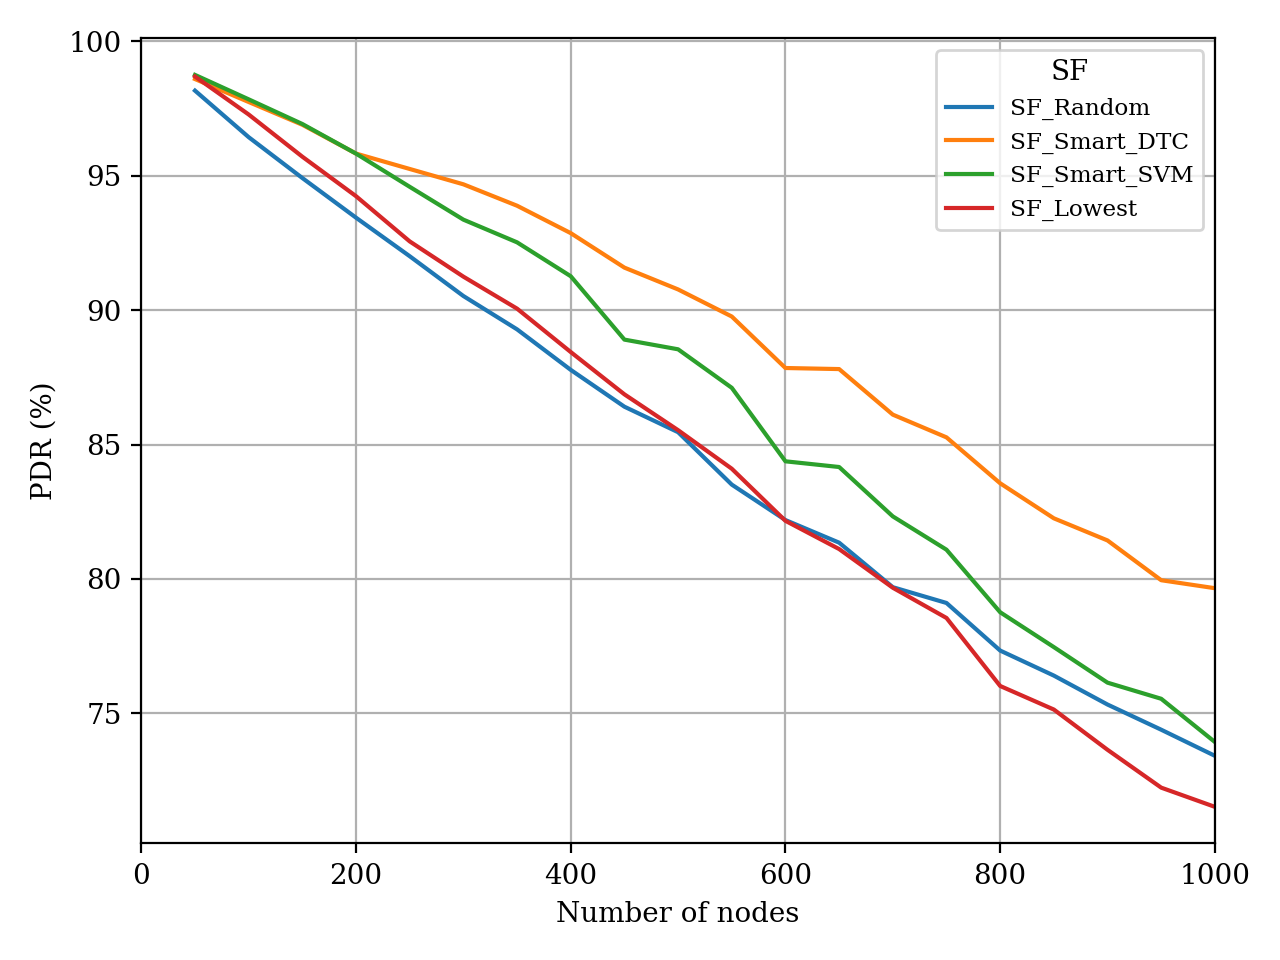
\includegraphics[width=.43\linewidth]{{fig/appendix/prediction_pdr_r5000_g3_p0.01_s3600}.png}}
\subfigure[Transmit energy]{
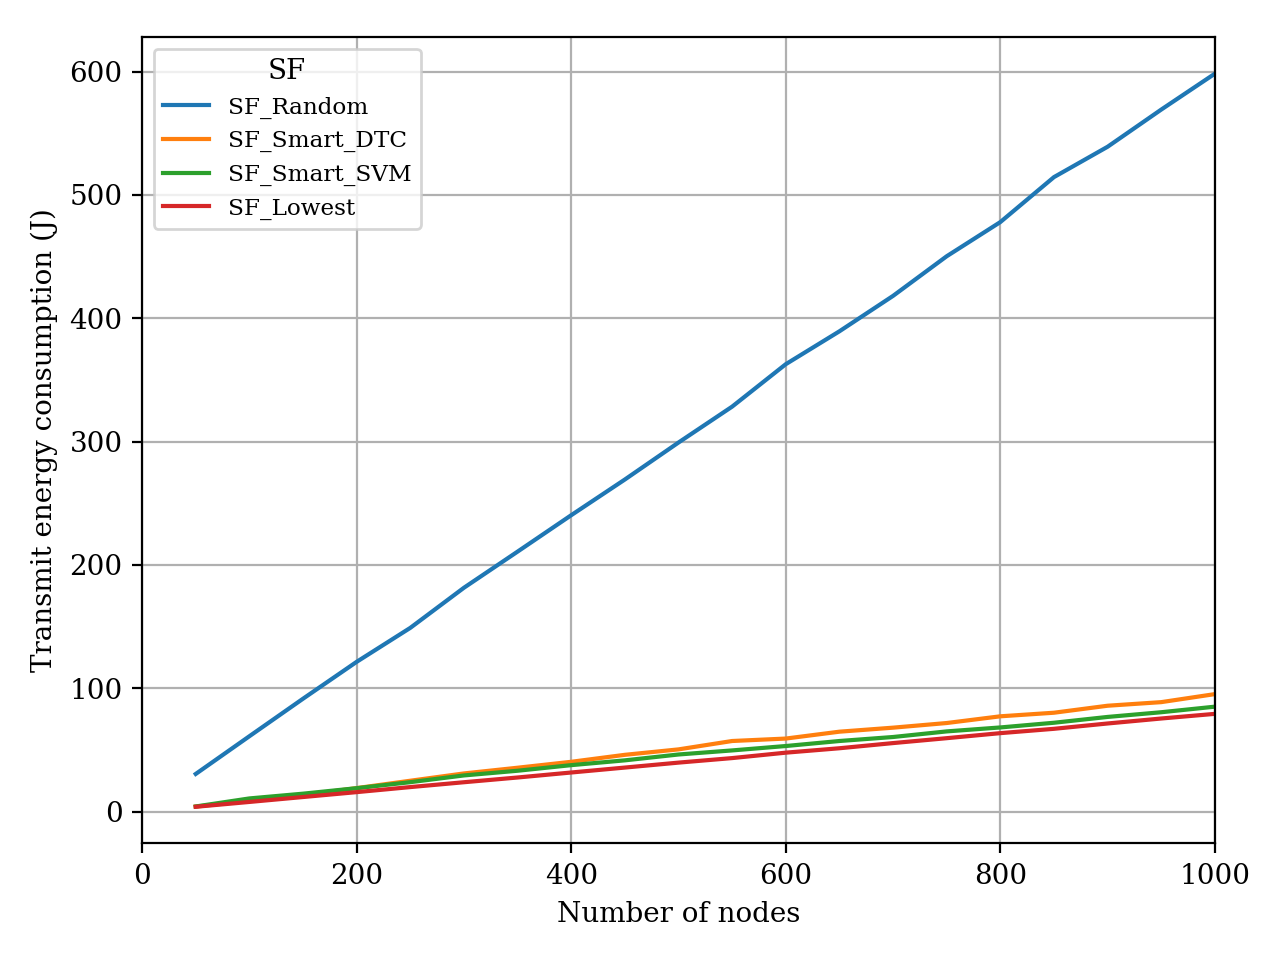
\includegraphics[width=.43\linewidth]{{fig/appendix/prediction_energy_r5000_g3_p0.01_s3600}.png}}
\caption{(r = 5000 m, GW = 3)}
\label{fig:prediction_r5000_g3}
\end{figure}

\begin{figure}[h]
\centering
\subfigure[PDR]{
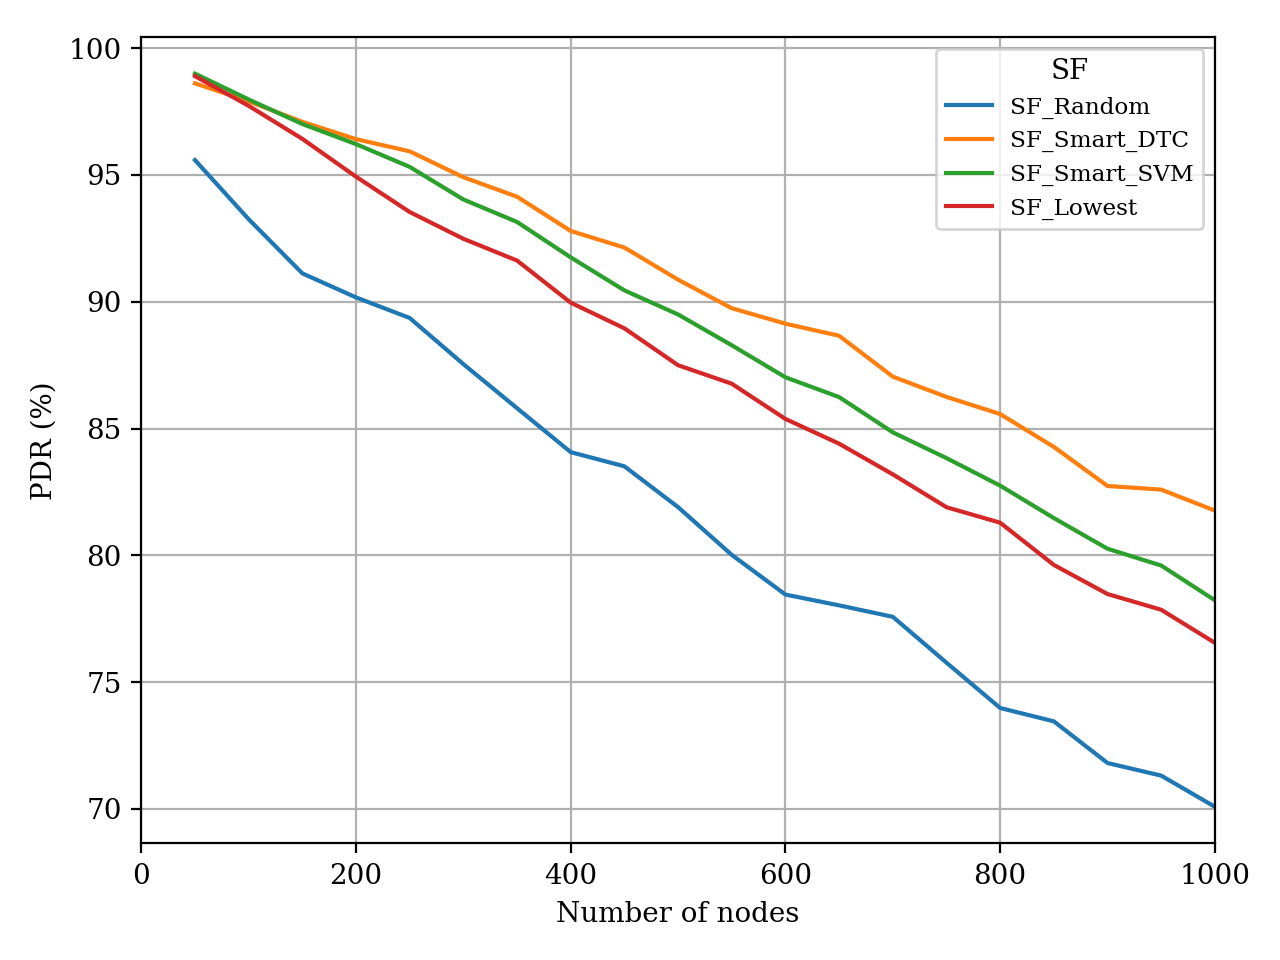
\includegraphics[width=.43\linewidth]{{fig/appendix/prediction_pdr_r7000_g3_p0.01_s3600}.png}}
\subfigure[Transmit energy]{
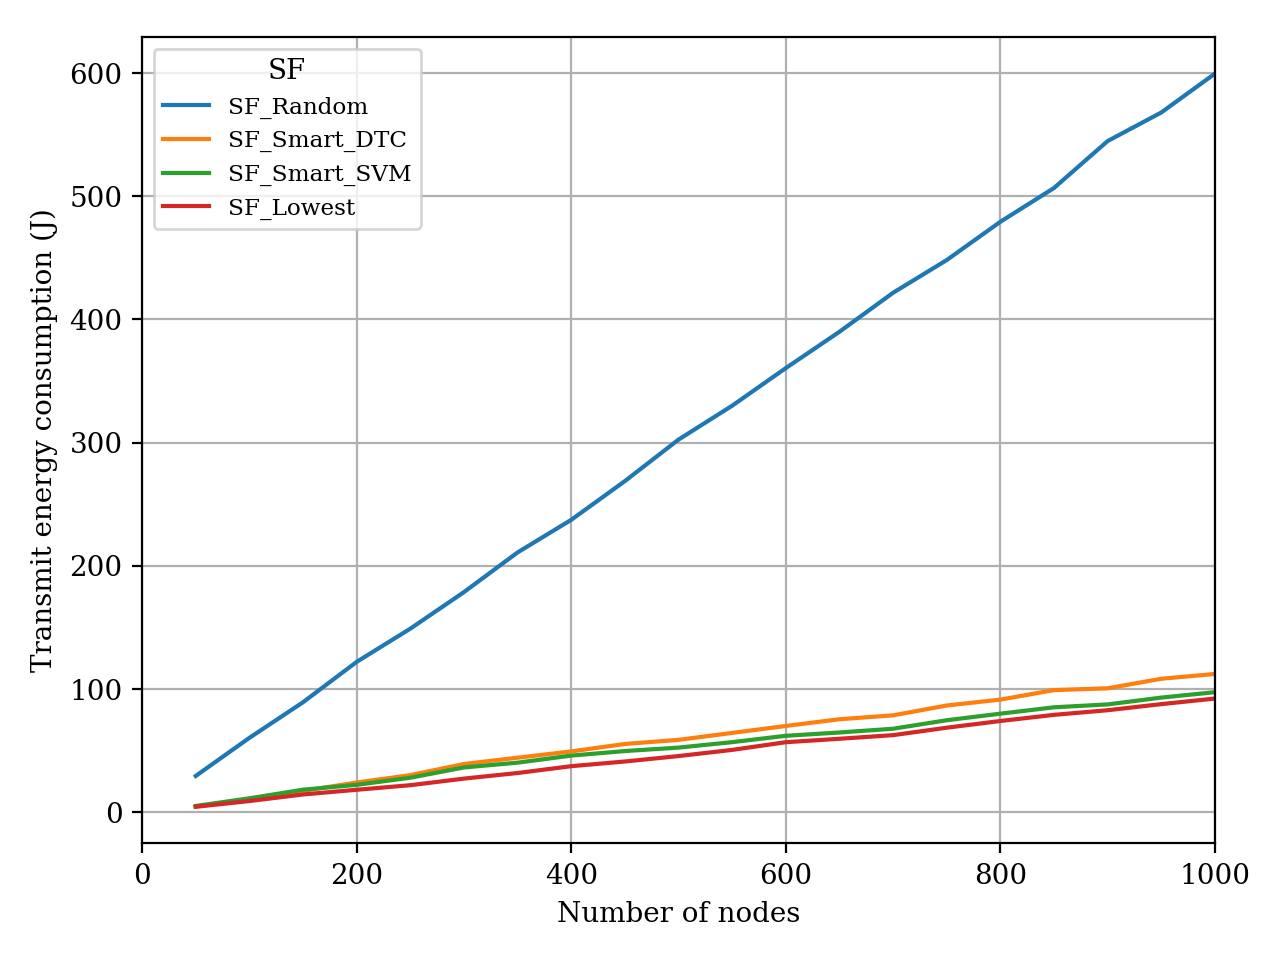
\includegraphics[width=.43\linewidth]{{fig/appendix/prediction_energy_r7000_g3_p0.01_s3600}.png}}
\caption{(r = 7000 m, GW = 3)}
\label{fig:prediction_r7000_g3}
\end{figure}

\begin{figure}[h]
\centering
\subfigure[PDR]{
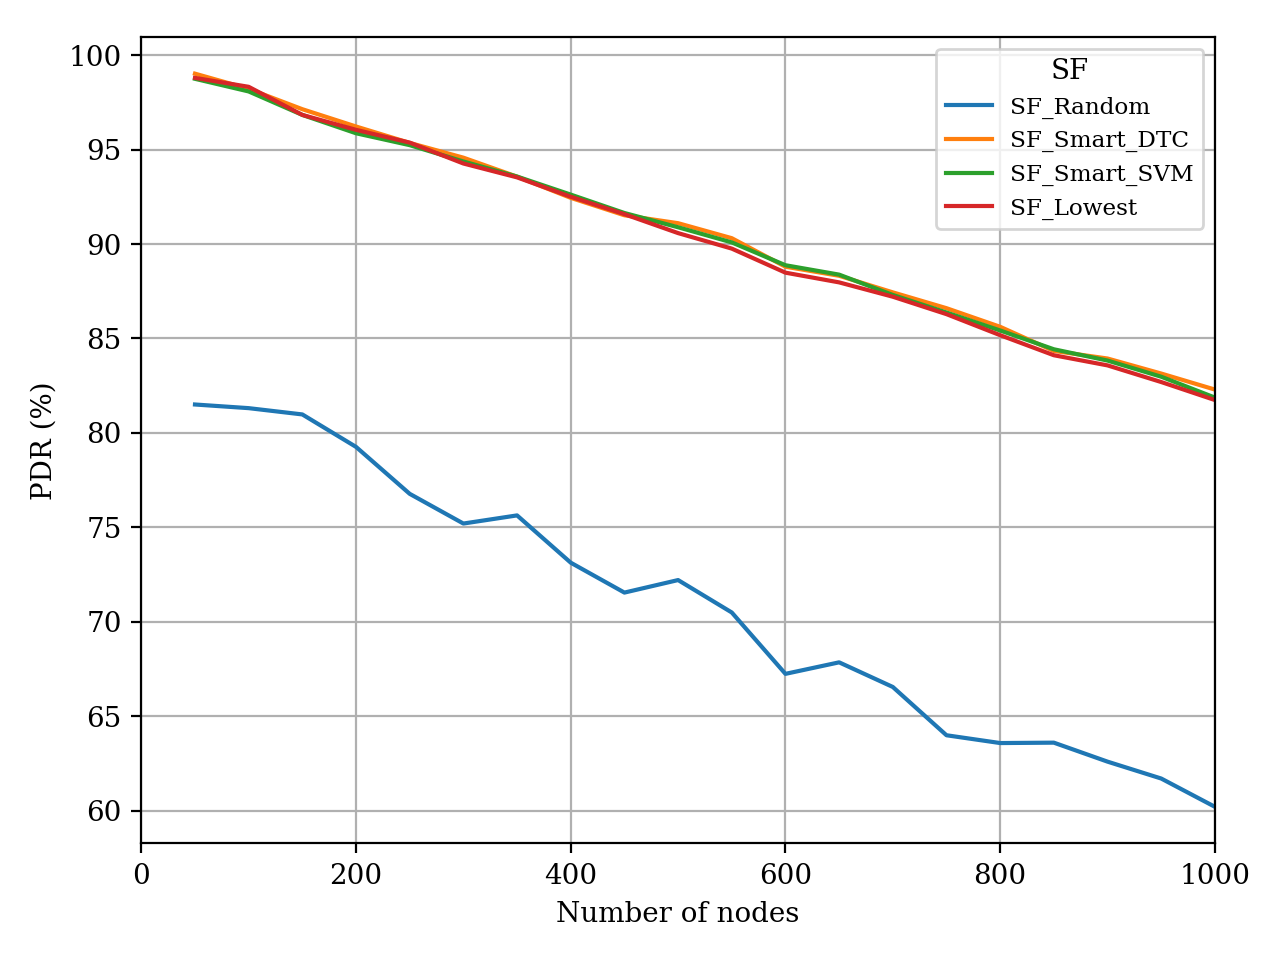
\includegraphics[width=.45\linewidth]{{fig/appendix/prediction_pdr_r10000_g3_p0.01_s3600}.png}}
\subfigure[Transmit energy]{
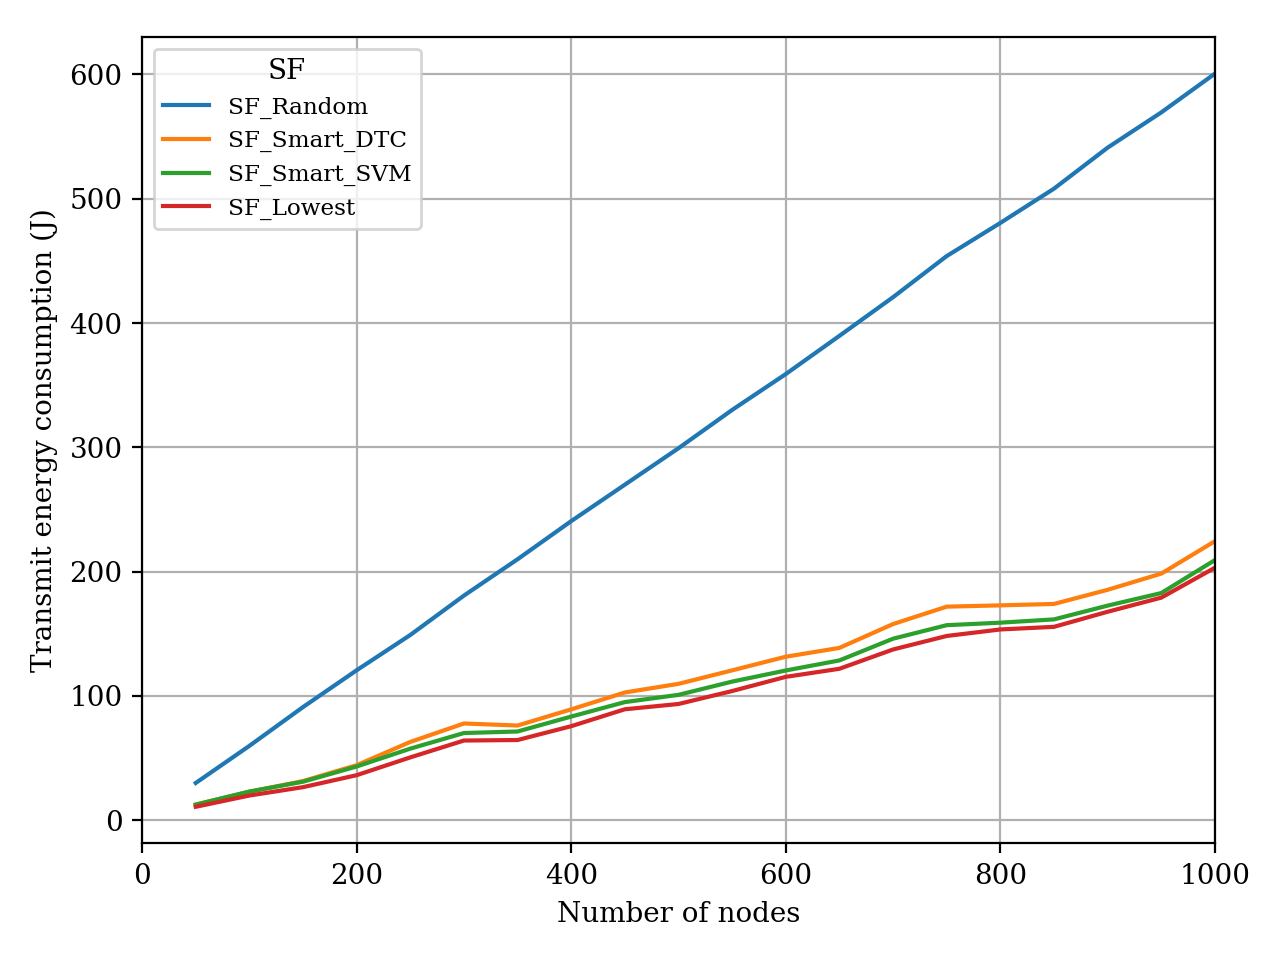
\includegraphics[width=.45\linewidth]{{fig/appendix/prediction_energy_r10000_g3_p0.01_s3600}.png}}
\caption{(r = 10000 m, GW = 3)}
\label{fig:prediction_r10000_g3}
\end{figure}


\begin{figure}[h]
\centering
\subfigure[PDR]{
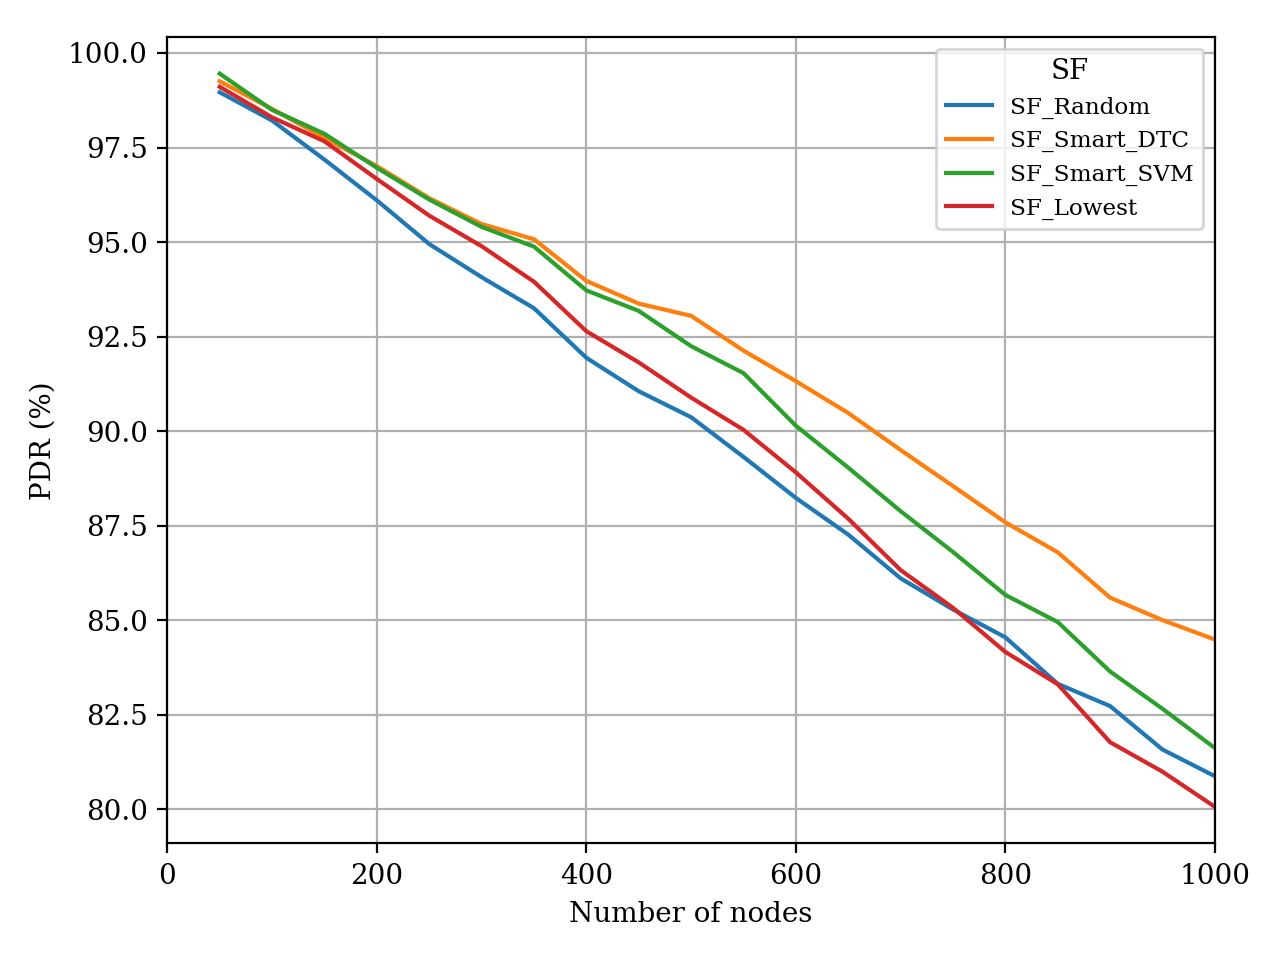
\includegraphics[width=.45\linewidth]{{fig/appendix/prediction_pdr_r3000_g4_p0.01_s3600}.png}}
\subfigure[Transmit energy]{
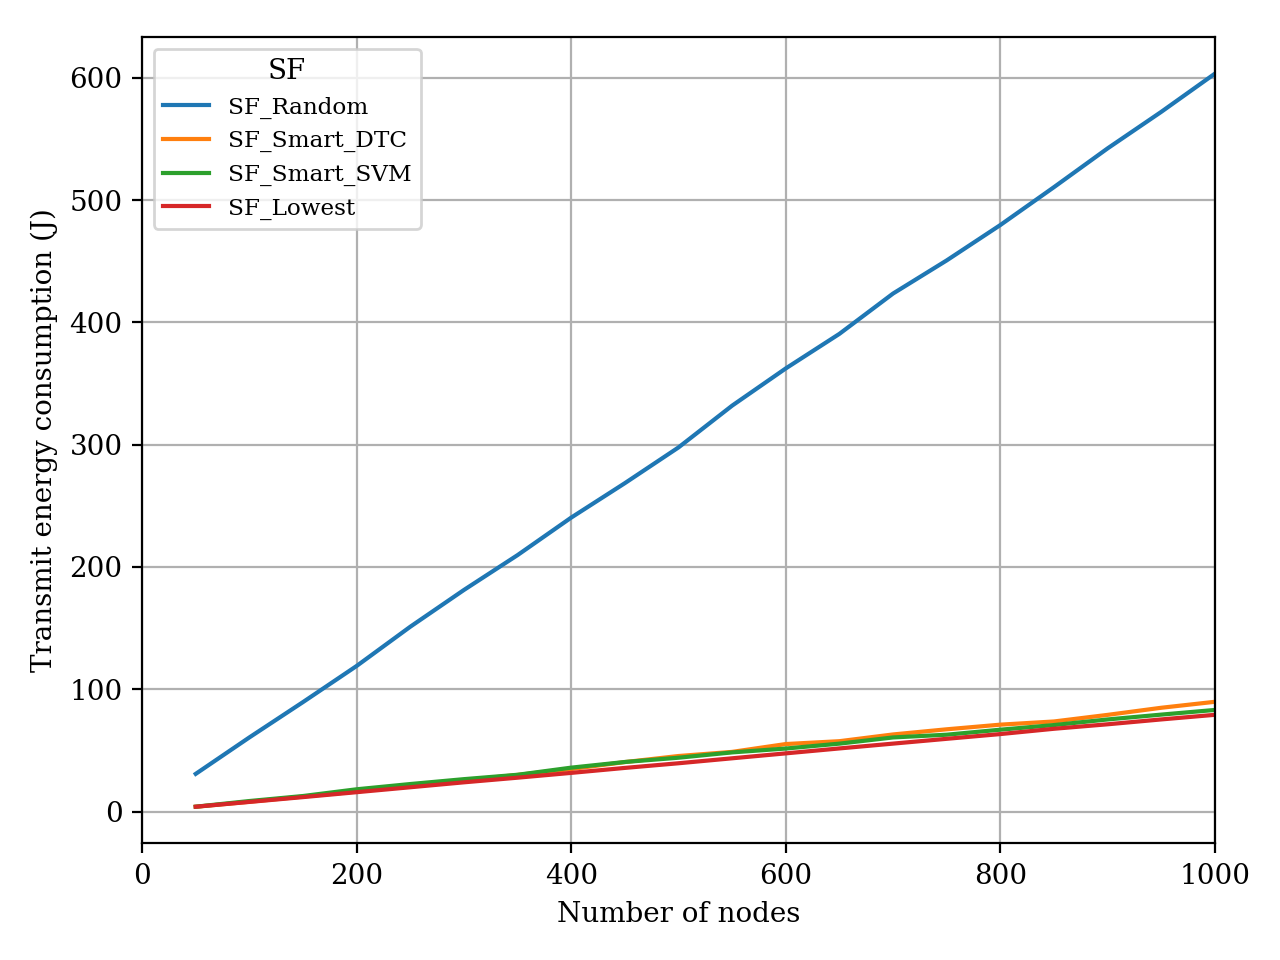
\includegraphics[width=.45\linewidth]{{fig/appendix/prediction_energy_r3000_g4_p0.01_s3600}.png}}
\caption{(r = 3000 m, GW = 4)}
\label{fig:prediction_r3000_g4}
\end{figure}

\begin{figure}[h]
\centering
\subfigure[PDR]{
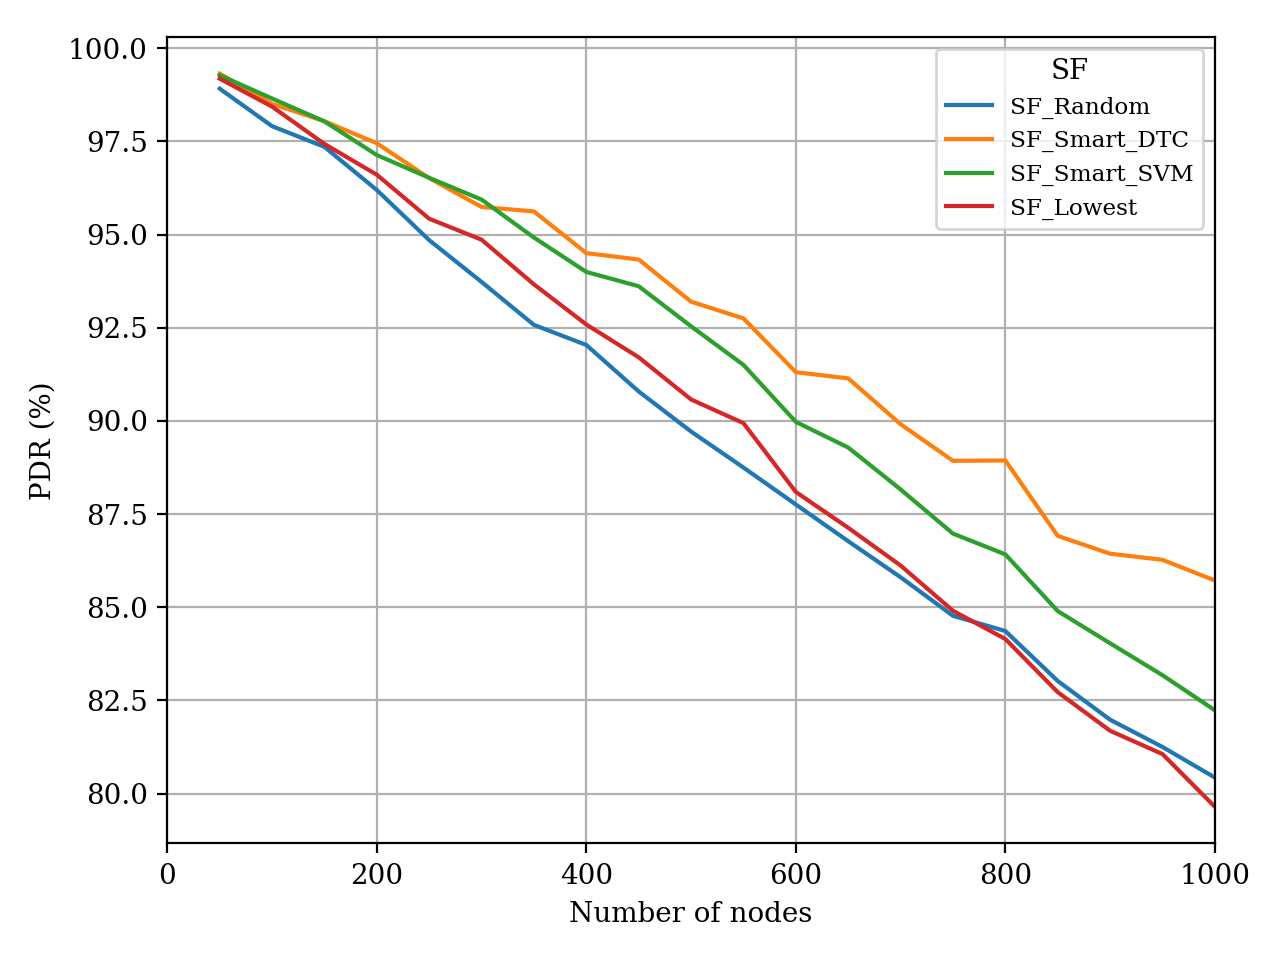
\includegraphics[width=.45\linewidth]{{fig/appendix/prediction_pdr_r5000_g4_p0.01_s3600}.png}}
\subfigure[Transmit energy]{
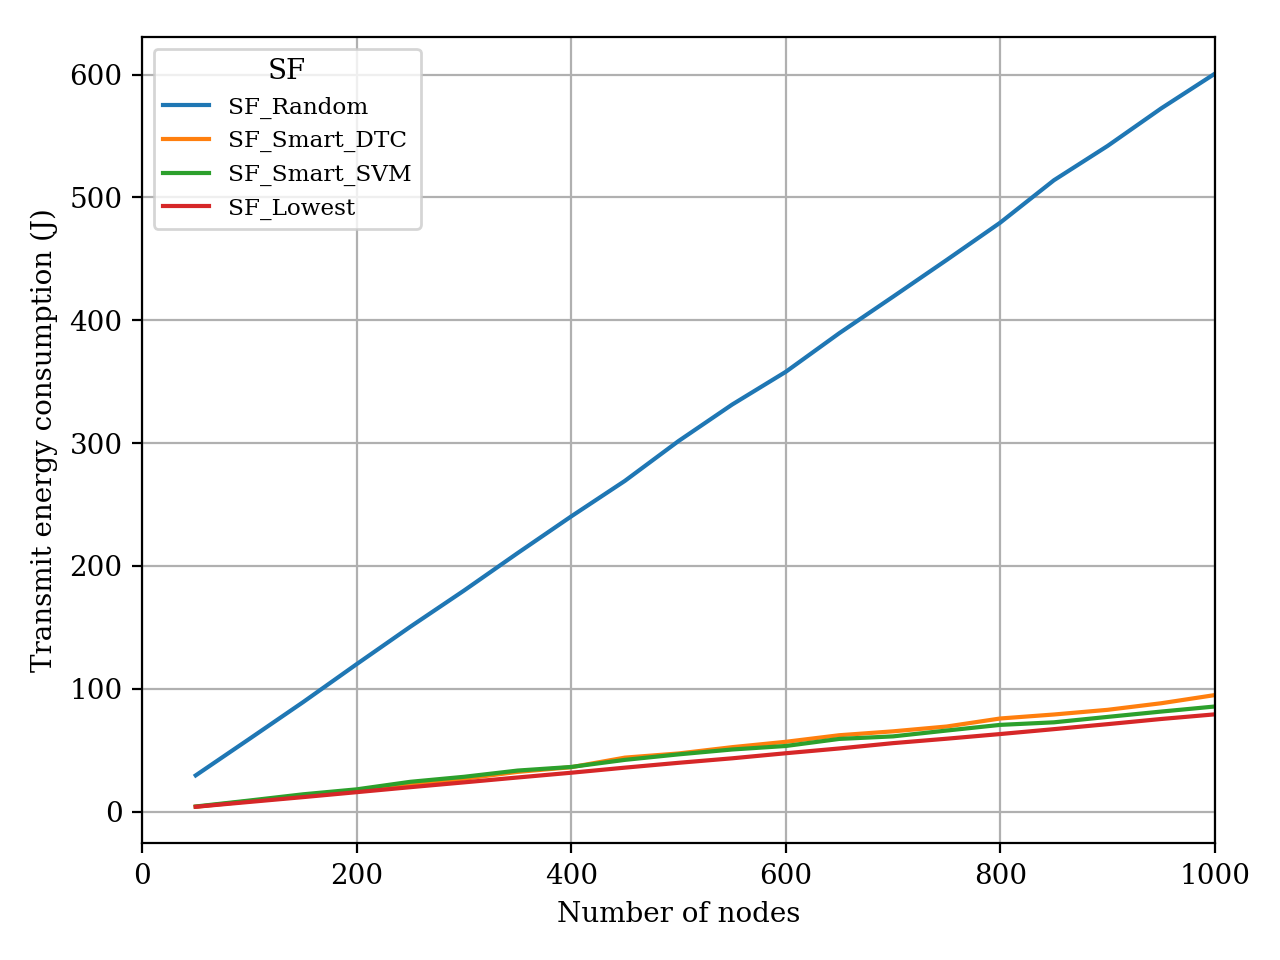
\includegraphics[width=.45\linewidth]{{fig/appendix/prediction_energy_r5000_g4_p0.01_s3600}.png}}
\caption{(r = 5000 m, GW = 4)}
\label{fig:prediction_r5000_g4}
\end{figure}

\begin{figure}[h]
\centering
\subfigure[PDR]{
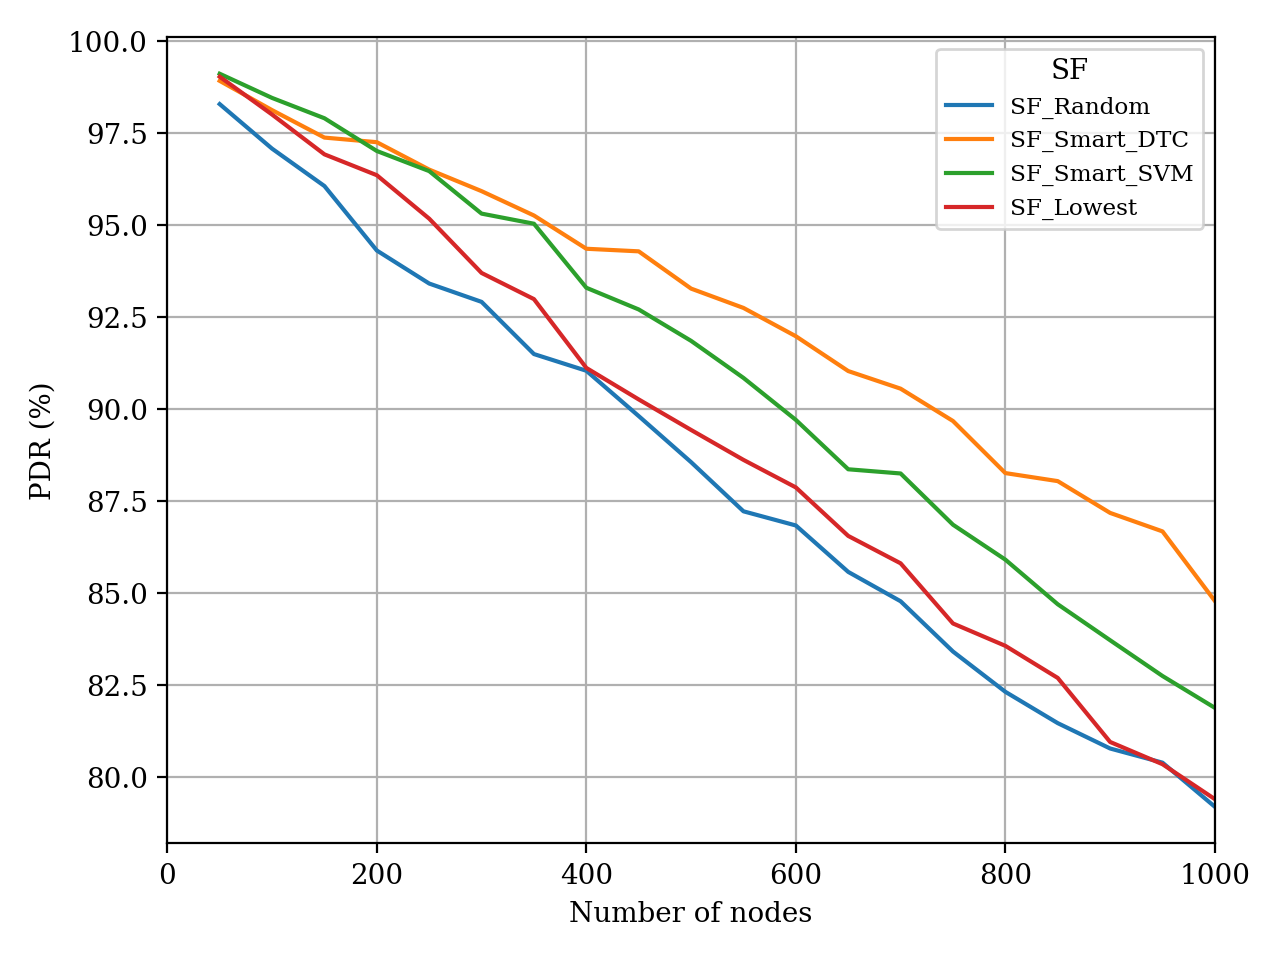
\includegraphics[width=.45\linewidth]{{fig/appendix/prediction_pdr_r7000_g4_p0.01_s3600}.png}}
\subfigure[Transmit enery]{
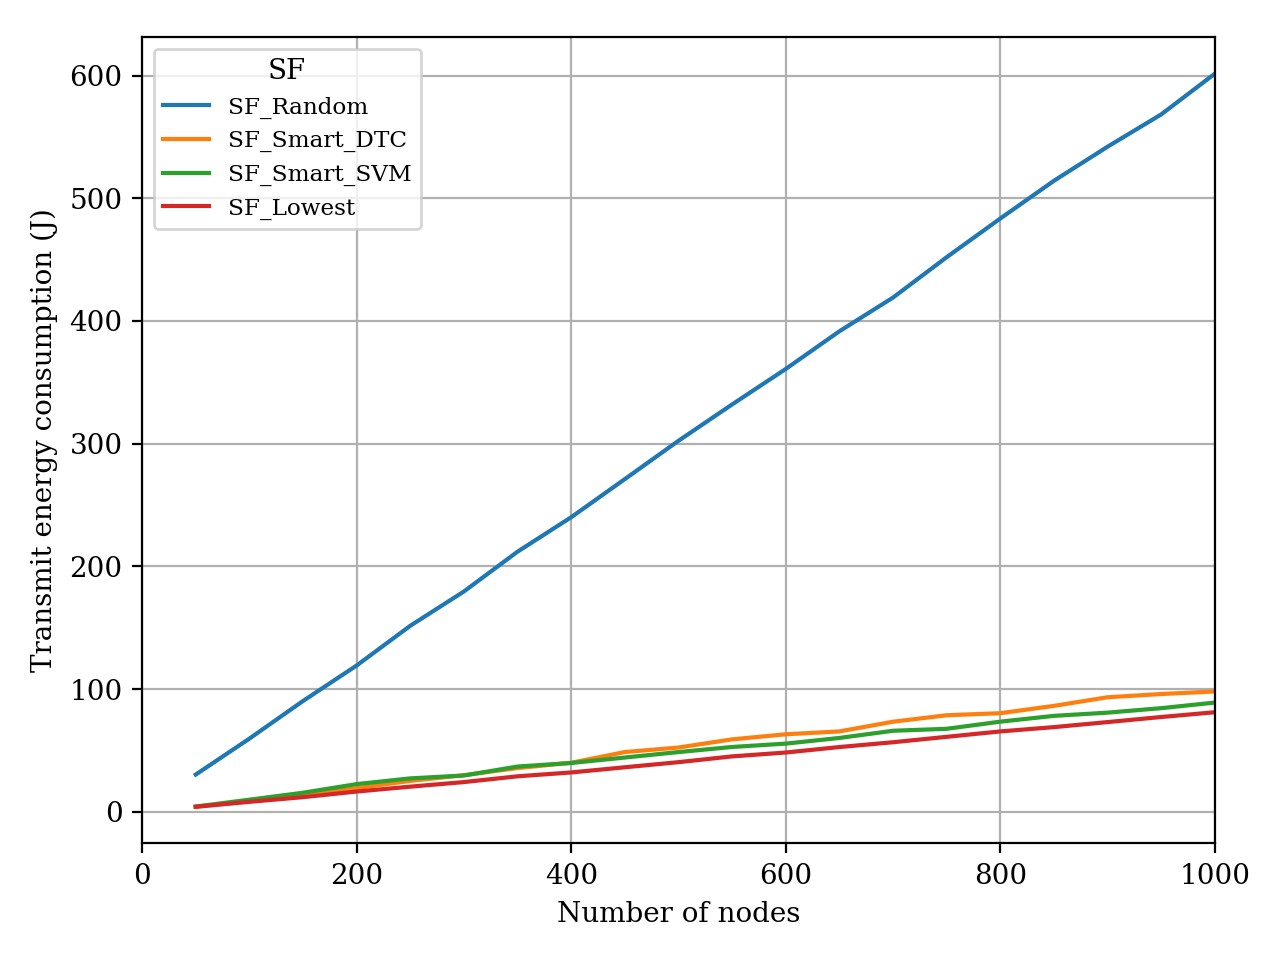
\includegraphics[width=.45\linewidth]{{fig/appendix/prediction_energy_r7000_g4_p0.01_s3600}.png}}
\caption{(r = 7000 m, GW = 4)}
\label{fig:prediction_r7000_g4}
\end{figure}

\begin{figure}[h]
\centering
\subfigure[PDR]{
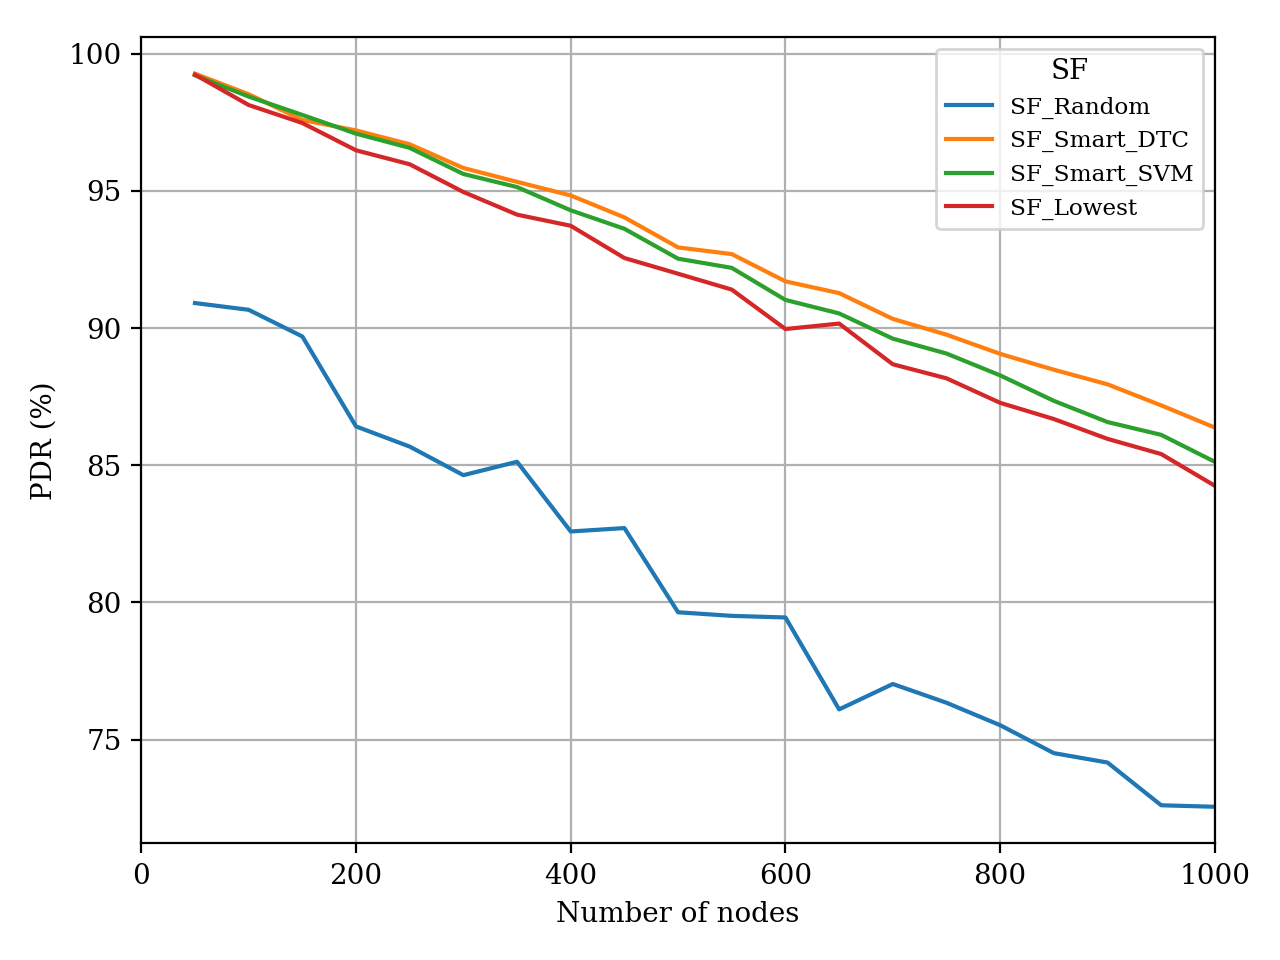
\includegraphics[width=.45\linewidth]{{fig/appendix/prediction_pdr_r10000_g4_p0.01_s3600}.png}}
\subfigure[Transmit energy]{
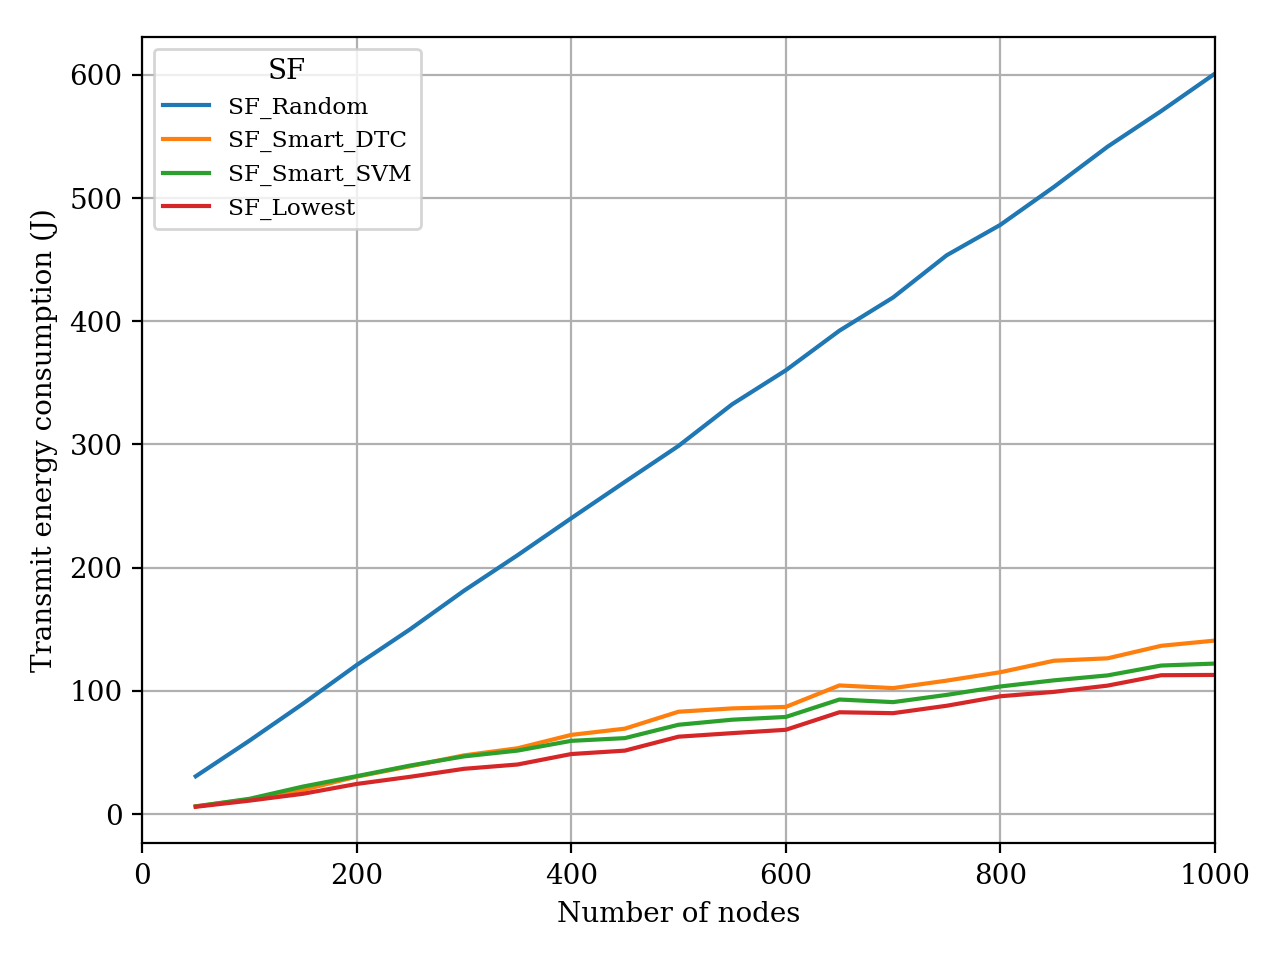
\includegraphics[width=.45\linewidth]{{fig/appendix/prediction_energy_r10000_g4_p0.01_s3600}.png}}
\caption{(r = 10000 m, GW = 4)}
\label{fig:prediction_r10000_g4}
\end{figure}
